\documentclass[12pt,openright,twoside]{report}
\usepackage[a4paper,top=25mm,bottom=25mm,right=25mm,left=25mm,bindingoffset=6mm]{geometry}
\usepackage[utf8]{inputenc}
\usepackage[swedish,british]{babel}
\usepackage{amsmath}
\usepackage{graphicx}
\usepackage[dvipsnames]{xcolor}
\usepackage{pict2e}
\usepackage{tabu}
\usepackage{booktabs}
%\usepackage{bookmark,hyperref}
\usepackage[hypertexnames=true]{hyperref}
%\usepackage{hyperref}
\usepackage{gensymb}
\usepackage{wrapfig}
\usepackage{multirow}
\usepackage[nottoc]{tocbibind}

\usepackage{xcolor}
\usepackage{colortbl}
%\usepackage[table]{xcolor}
%\usepackage{tabularray}
\usepackage{watermark}
\usepackage{wallpaper}
\usepackage{eurosym}
\usepackage[toc,title,page]{appendix}
\usepackage{courier}
\usepackage{listings} 
\usepackage{enumitem}
\usepackage{url}
\usepackage{soul}
\usepackage{comment}
\usepackage{parskip}
\usepackage{etoolbox}
\usepackage{float}
\usepackage[T1]{fontenc}
%\usepackage{fontspec}
\graphicspath{{figuren/}}
\usepackage{tikz}
\usetikzlibrary{shapes.geometric, arrows, positioning, fit}


\definecolor{mygray}{gray}{0.85}

\newcommand{\ctext}[3][RGB]{%
	\begingroup
	\definecolor{hlcolor}{#1}{#2}\sethlcolor{hlcolor}%
	\hl{#3}%
	\endgroup
}


\newcommand{\specialcell}[2][c]{%
	\begin{tabular}[#1]{@{}c@{}}#2\end{tabular}}

\newcommand*{\img}[1]{%
	\raisebox{-.3\baselineskip}{%
		\includegraphics[
		height=\baselineskip,
		width=\baselineskip,
		keepaspectratio,
		]{#1}%
	}%
}


 %%%%%%%%%%%%%%%%%%%%%%%%%%%%%%%%%%%%%%%%%%%%%%%%%%%%%%%%%%%%%%%%%%%%%%%%%%%%%%%% 
%%% ~ Arduino Language - Arduino IDE Colors ~                                  %%%
%%%                                                                            %%%
%%% Kyle Rocha-Brownell | 10/2/2017 | No Licence                               %%%
%%% -------------------------------------------------------------------------- %%%
%%%                                                                            %%%
%%% Place this file in your working directory (next to the latex file you're   %%%
%%% working on).  To add it to your project, place:                            %%%
%%%     %%%%%%%%%%%%%%%%%%%%%%%%%%%%%%%%%%%%%%%%%%%%%%%%%%%%%%%%%%%%%%%%%%%%%%%%%%%%%%%% 
%%% ~ Arduino Language - Arduino IDE Colors ~                                  %%%
%%%                                                                            %%%
%%% Kyle Rocha-Brownell | 10/2/2017 | No Licence                               %%%
%%% -------------------------------------------------------------------------- %%%
%%%                                                                            %%%
%%% Place this file in your working directory (next to the latex file you're   %%%
%%% working on).  To add it to your project, place:                            %%%
%%%     %%%%%%%%%%%%%%%%%%%%%%%%%%%%%%%%%%%%%%%%%%%%%%%%%%%%%%%%%%%%%%%%%%%%%%%%%%%%%%%% 
%%% ~ Arduino Language - Arduino IDE Colors ~                                  %%%
%%%                                                                            %%%
%%% Kyle Rocha-Brownell | 10/2/2017 | No Licence                               %%%
%%% -------------------------------------------------------------------------- %%%
%%%                                                                            %%%
%%% Place this file in your working directory (next to the latex file you're   %%%
%%% working on).  To add it to your project, place:                            %%%
%%%    \input{arduinoLanguage.tex}                                             %%%
%%% somewhere before \begin{document} in your latex file.                      %%%
%%%                                                                            %%%
%%% In your document, place your arduino code between:                         %%%
%%%   \begin{lstlisting}[language=Arduino]                                     %%%
%%% and:                                                                       %%%
%%%   \end{lstlisting}                                                         %%%
%%%                                                                            %%%
%%% Or create your own style to add non-built-in functions and variables.      %%%
%%%                                                                            %%%
 %%%%%%%%%%%%%%%%%%%%%%%%%%%%%%%%%%%%%%%%%%%%%%%%%%%%%%%%%%%%%%%%%%%%%%%%%%%%%%%% 

\usepackage{color}
\usepackage{listings}    
\usepackage{courier}

%%% Define Custom IDE Colors %%%
\definecolor{arduinoGreen}    {rgb} {0.17, 0.43, 0.01}
\definecolor{arduinoGrey}     {rgb} {0.47, 0.47, 0.33}
\definecolor{arduinoOrange}   {rgb} {0.8 , 0.4 , 0   }
\definecolor{arduinoBlue}     {rgb} {0.01, 0.61, 0.98}
\definecolor{arduinoDarkBlue} {rgb} {0.0 , 0.2 , 0.5 }

%%% Define Arduino Language %%%
\lstdefinelanguage{Arduino}{
  language=C++, % begin with default C++ settings 
%
%
  %%% Keyword Color Group 1 %%%  (called KEYWORD3 by arduino)
  keywordstyle=\color{arduinoGreen},   
  deletekeywords={  % remove all arduino keywords that might be in c++
                break, case, override, final, continue, default, do, else, for, 
                if, return, goto, switch, throw, try, while, setup, loop, export, 
                not, or, and, xor, include, define, elif, else, error, if, ifdef, 
                ifndef, pragma, warning,
                HIGH, LOW, INPUT, INPUT_PULLUP, OUTPUT, DEC, BIN, HEX, OCT, PI, 
                HALF_PI, TWO_PI, LSBFIRST, MSBFIRST, CHANGE, FALLING, RISING, 
                DEFAULT, EXTERNAL, INTERNAL, INTERNAL1V1, INTERNAL2V56, LED_BUILTIN, 
                LED_BUILTIN_RX, LED_BUILTIN_TX, DIGITAL_MESSAGE, FIRMATA_STRING, 
                ANALOG_MESSAGE, REPORT_DIGITAL, REPORT_ANALOG, SET_PIN_MODE, 
                SYSTEM_RESET, SYSEX_START, auto, int8_t, int16_t, int32_t, int64_t, 
                uint8_t, uint16_t, uint32_t, uint64_t, char16_t, char32_t, operator, 
                enum, delete, bool, boolean, byte, char, const, false, float, double, 
                null, NULL, int, long, new, private, protected, public, short, 
                signed, static, volatile, String, void, true, unsigned, word, array, 
                sizeof, dynamic_cast, typedef, const_cast, struct, static_cast, union, 
                friend, extern, class, reinterpret_cast, register, explicit, inline, 
                _Bool, complex, _Complex, _Imaginary, atomic_bool, atomic_char, 
                atomic_schar, atomic_uchar, atomic_short, atomic_ushort, atomic_int, 
                atomic_uint, atomic_long, atomic_ulong, atomic_llong, atomic_ullong, 
                virtual, PROGMEM,
                Serial, Serial1, Serial2, Serial3, SerialUSB, Keyboard, Mouse,
                abs, acos, asin, atan, atan2, ceil, constrain, cos, degrees, exp, 
                floor, log, map, max, min, radians, random, randomSeed, round, sin, 
                sq, sqrt, tan, pow, bitRead, bitWrite, bitSet, bitClear, bit, 
                highByte, lowByte, analogReference, analogRead, 
                analogReadResolution, analogWrite, analogWriteResolution, 
                attachInterrupt, detachInterrupt, digitalPinToInterrupt, delay, 
                delayMicroseconds, digitalWrite, digitalRead, interrupts, millis, 
                micros, noInterrupts, noTone, pinMode, pulseIn, pulseInLong, shiftIn, 
                shiftOut, tone, yield, Stream, begin, end, peek, read, print, 
                println, available, availableForWrite, flush, setTimeout, find, 
                findUntil, parseInt, parseFloat, readBytes, readBytesUntil, readString, 
                readStringUntil, trim, toUpperCase, toLowerCase, charAt, compareTo, 
                concat, endsWith, startsWith, equals, equalsIgnoreCase, getBytes, 
                indexOf, lastIndexOf, length, replace, setCharAt, substring, 
                toCharArray, toInt, press, release, releaseAll, accept, click, move, 
                isPressed, isAlphaNumeric, isAlpha, isAscii, isWhitespace, isControl, 
                isDigit, isGraph, isLowerCase, isPrintable, isPunct, isSpace, 
                isUpperCase, isHexadecimalDigit, 
                }, 
  morekeywords={   % add arduino structures to group 1
                break, case, override, final, continue, default, do, else, for, 
                if, return, goto, switch, throw, try, while, setup, loop, export, 
                not, or, and, xor, include, define, elif, else, error, if, ifdef, 
                ifndef, pragma, warning,
                }, 
% 
%
  %%% Keyword Color Group 2 %%%  (called LITERAL1 by arduino)
  keywordstyle=[2]\color{arduinoBlue},   
  keywords=[2]{   % add variables and dataTypes as 2nd group  
                HIGH, LOW, INPUT, INPUT_PULLUP, OUTPUT, DEC, BIN, HEX, OCT, PI, 
                HALF_PI, TWO_PI, LSBFIRST, MSBFIRST, CHANGE, FALLING, RISING, 
                DEFAULT, EXTERNAL, INTERNAL, INTERNAL1V1, INTERNAL2V56, LED_BUILTIN, 
                LED_BUILTIN_RX, LED_BUILTIN_TX, DIGITAL_MESSAGE, FIRMATA_STRING, 
                ANALOG_MESSAGE, REPORT_DIGITAL, REPORT_ANALOG, SET_PIN_MODE, 
                SYSTEM_RESET, SYSEX_START, auto, int8_t, int16_t, int32_t, int64_t, 
                uint8_t, uint16_t, uint32_t, uint64_t, char16_t, char32_t, operator, 
                enum, delete, bool, boolean, byte, char, const, false, float, double, 
                null, NULL, int, long, new, private, protected, public, short, 
                signed, static, volatile, String, void, true, unsigned, word, array, 
                sizeof, dynamic_cast, typedef, const_cast, struct, static_cast, union, 
                friend, extern, class, reinterpret_cast, register, explicit, inline, 
                _Bool, complex, _Complex, _Imaginary, atomic_bool, atomic_char, 
                atomic_schar, atomic_uchar, atomic_short, atomic_ushort, atomic_int, 
                atomic_uint, atomic_long, atomic_ulong, atomic_llong, atomic_ullong, 
                virtual, PROGMEM,
                },  
% 
%
  %%% Keyword Color Group 3 %%%  (called KEYWORD1 by arduino)
  keywordstyle=[3]\bfseries\color{arduinoOrange},
  keywords=[3]{  % add built-in functions as a 3rd group
                Serial, Serial1, Serial2, Serial3, SerialUSB, Keyboard, Mouse,
                },      
%
%
  %%% Keyword Color Group 4 %%%  (called KEYWORD2 by arduino)
  keywordstyle=[4]\color{arduinoOrange},
  keywords=[4]{  % add more built-in functions as a 4th group
                abs, acos, asin, atan, atan2, ceil, constrain, cos, degrees, exp, 
                floor, log, map, max, min, radians, random, randomSeed, round, sin, 
                sq, sqrt, tan, pow, bitRead, bitWrite, bitSet, bitClear, bit, 
                highByte, lowByte, analogReference, analogRead, 
                analogReadResolution, analogWrite, analogWriteResolution, 
                attachInterrupt, detachInterrupt, digitalPinToInterrupt, delay, 
                delayMicroseconds, digitalWrite, digitalRead, interrupts, millis, 
                micros, noInterrupts, noTone, pinMode, pulseIn, pulseInLong, shiftIn, 
                shiftOut, tone, yield, Stream, begin, end, peek, read, print, 
                println, available, availableForWrite, flush, setTimeout, find, 
                findUntil, parseInt, parseFloat, readBytes, readBytesUntil, readString, 
                readStringUntil, trim, toUpperCase, toLowerCase, charAt, compareTo, 
                concat, endsWith, startsWith, equals, equalsIgnoreCase, getBytes, 
                indexOf, lastIndexOf, length, replace, setCharAt, substring, 
                toCharArray, toInt, press, release, releaseAll, accept, click, move, 
                isPressed, isAlphaNumeric, isAlpha, isAscii, isWhitespace, isControl, 
                isDigit, isGraph, isLowerCase, isPrintable, isPunct, isSpace, 
                isUpperCase, isHexadecimalDigit, 
                },      
%
%
  %%% Set Other Colors %%%
  stringstyle=\color{arduinoDarkBlue},    
  commentstyle=\color{arduinoGrey},    
%          
%   
  %%%% Line Numbering %%%%
  numbers=left,                    
  numbersep=5pt,                   
  numberstyle=\color{arduinoGrey},    
  %stepnumber=2,                      % show every 2 line numbers
%
%
  %%%% Code Box Style %%%%
  breaklines=true,                    % wordwrapping
  tabsize=2,         
  basicstyle=\ttfamily  
}
                                             %%%
%%% somewhere before \begin{document} in your latex file.                      %%%
%%%                                                                            %%%
%%% In your document, place your arduino code between:                         %%%
%%%   \begin{lstlisting}[language=Arduino]                                     %%%
%%% and:                                                                       %%%
%%%   \end{lstlisting}                                                         %%%
%%%                                                                            %%%
%%% Or create your own style to add non-built-in functions and variables.      %%%
%%%                                                                            %%%
 %%%%%%%%%%%%%%%%%%%%%%%%%%%%%%%%%%%%%%%%%%%%%%%%%%%%%%%%%%%%%%%%%%%%%%%%%%%%%%%% 

\usepackage{color}
\usepackage{listings}    
\usepackage{courier}

%%% Define Custom IDE Colors %%%
\definecolor{arduinoGreen}    {rgb} {0.17, 0.43, 0.01}
\definecolor{arduinoGrey}     {rgb} {0.47, 0.47, 0.33}
\definecolor{arduinoOrange}   {rgb} {0.8 , 0.4 , 0   }
\definecolor{arduinoBlue}     {rgb} {0.01, 0.61, 0.98}
\definecolor{arduinoDarkBlue} {rgb} {0.0 , 0.2 , 0.5 }

%%% Define Arduino Language %%%
\lstdefinelanguage{Arduino}{
  language=C++, % begin with default C++ settings 
%
%
  %%% Keyword Color Group 1 %%%  (called KEYWORD3 by arduino)
  keywordstyle=\color{arduinoGreen},   
  deletekeywords={  % remove all arduino keywords that might be in c++
                break, case, override, final, continue, default, do, else, for, 
                if, return, goto, switch, throw, try, while, setup, loop, export, 
                not, or, and, xor, include, define, elif, else, error, if, ifdef, 
                ifndef, pragma, warning,
                HIGH, LOW, INPUT, INPUT_PULLUP, OUTPUT, DEC, BIN, HEX, OCT, PI, 
                HALF_PI, TWO_PI, LSBFIRST, MSBFIRST, CHANGE, FALLING, RISING, 
                DEFAULT, EXTERNAL, INTERNAL, INTERNAL1V1, INTERNAL2V56, LED_BUILTIN, 
                LED_BUILTIN_RX, LED_BUILTIN_TX, DIGITAL_MESSAGE, FIRMATA_STRING, 
                ANALOG_MESSAGE, REPORT_DIGITAL, REPORT_ANALOG, SET_PIN_MODE, 
                SYSTEM_RESET, SYSEX_START, auto, int8_t, int16_t, int32_t, int64_t, 
                uint8_t, uint16_t, uint32_t, uint64_t, char16_t, char32_t, operator, 
                enum, delete, bool, boolean, byte, char, const, false, float, double, 
                null, NULL, int, long, new, private, protected, public, short, 
                signed, static, volatile, String, void, true, unsigned, word, array, 
                sizeof, dynamic_cast, typedef, const_cast, struct, static_cast, union, 
                friend, extern, class, reinterpret_cast, register, explicit, inline, 
                _Bool, complex, _Complex, _Imaginary, atomic_bool, atomic_char, 
                atomic_schar, atomic_uchar, atomic_short, atomic_ushort, atomic_int, 
                atomic_uint, atomic_long, atomic_ulong, atomic_llong, atomic_ullong, 
                virtual, PROGMEM,
                Serial, Serial1, Serial2, Serial3, SerialUSB, Keyboard, Mouse,
                abs, acos, asin, atan, atan2, ceil, constrain, cos, degrees, exp, 
                floor, log, map, max, min, radians, random, randomSeed, round, sin, 
                sq, sqrt, tan, pow, bitRead, bitWrite, bitSet, bitClear, bit, 
                highByte, lowByte, analogReference, analogRead, 
                analogReadResolution, analogWrite, analogWriteResolution, 
                attachInterrupt, detachInterrupt, digitalPinToInterrupt, delay, 
                delayMicroseconds, digitalWrite, digitalRead, interrupts, millis, 
                micros, noInterrupts, noTone, pinMode, pulseIn, pulseInLong, shiftIn, 
                shiftOut, tone, yield, Stream, begin, end, peek, read, print, 
                println, available, availableForWrite, flush, setTimeout, find, 
                findUntil, parseInt, parseFloat, readBytes, readBytesUntil, readString, 
                readStringUntil, trim, toUpperCase, toLowerCase, charAt, compareTo, 
                concat, endsWith, startsWith, equals, equalsIgnoreCase, getBytes, 
                indexOf, lastIndexOf, length, replace, setCharAt, substring, 
                toCharArray, toInt, press, release, releaseAll, accept, click, move, 
                isPressed, isAlphaNumeric, isAlpha, isAscii, isWhitespace, isControl, 
                isDigit, isGraph, isLowerCase, isPrintable, isPunct, isSpace, 
                isUpperCase, isHexadecimalDigit, 
                }, 
  morekeywords={   % add arduino structures to group 1
                break, case, override, final, continue, default, do, else, for, 
                if, return, goto, switch, throw, try, while, setup, loop, export, 
                not, or, and, xor, include, define, elif, else, error, if, ifdef, 
                ifndef, pragma, warning,
                }, 
% 
%
  %%% Keyword Color Group 2 %%%  (called LITERAL1 by arduino)
  keywordstyle=[2]\color{arduinoBlue},   
  keywords=[2]{   % add variables and dataTypes as 2nd group  
                HIGH, LOW, INPUT, INPUT_PULLUP, OUTPUT, DEC, BIN, HEX, OCT, PI, 
                HALF_PI, TWO_PI, LSBFIRST, MSBFIRST, CHANGE, FALLING, RISING, 
                DEFAULT, EXTERNAL, INTERNAL, INTERNAL1V1, INTERNAL2V56, LED_BUILTIN, 
                LED_BUILTIN_RX, LED_BUILTIN_TX, DIGITAL_MESSAGE, FIRMATA_STRING, 
                ANALOG_MESSAGE, REPORT_DIGITAL, REPORT_ANALOG, SET_PIN_MODE, 
                SYSTEM_RESET, SYSEX_START, auto, int8_t, int16_t, int32_t, int64_t, 
                uint8_t, uint16_t, uint32_t, uint64_t, char16_t, char32_t, operator, 
                enum, delete, bool, boolean, byte, char, const, false, float, double, 
                null, NULL, int, long, new, private, protected, public, short, 
                signed, static, volatile, String, void, true, unsigned, word, array, 
                sizeof, dynamic_cast, typedef, const_cast, struct, static_cast, union, 
                friend, extern, class, reinterpret_cast, register, explicit, inline, 
                _Bool, complex, _Complex, _Imaginary, atomic_bool, atomic_char, 
                atomic_schar, atomic_uchar, atomic_short, atomic_ushort, atomic_int, 
                atomic_uint, atomic_long, atomic_ulong, atomic_llong, atomic_ullong, 
                virtual, PROGMEM,
                },  
% 
%
  %%% Keyword Color Group 3 %%%  (called KEYWORD1 by arduino)
  keywordstyle=[3]\bfseries\color{arduinoOrange},
  keywords=[3]{  % add built-in functions as a 3rd group
                Serial, Serial1, Serial2, Serial3, SerialUSB, Keyboard, Mouse,
                },      
%
%
  %%% Keyword Color Group 4 %%%  (called KEYWORD2 by arduino)
  keywordstyle=[4]\color{arduinoOrange},
  keywords=[4]{  % add more built-in functions as a 4th group
                abs, acos, asin, atan, atan2, ceil, constrain, cos, degrees, exp, 
                floor, log, map, max, min, radians, random, randomSeed, round, sin, 
                sq, sqrt, tan, pow, bitRead, bitWrite, bitSet, bitClear, bit, 
                highByte, lowByte, analogReference, analogRead, 
                analogReadResolution, analogWrite, analogWriteResolution, 
                attachInterrupt, detachInterrupt, digitalPinToInterrupt, delay, 
                delayMicroseconds, digitalWrite, digitalRead, interrupts, millis, 
                micros, noInterrupts, noTone, pinMode, pulseIn, pulseInLong, shiftIn, 
                shiftOut, tone, yield, Stream, begin, end, peek, read, print, 
                println, available, availableForWrite, flush, setTimeout, find, 
                findUntil, parseInt, parseFloat, readBytes, readBytesUntil, readString, 
                readStringUntil, trim, toUpperCase, toLowerCase, charAt, compareTo, 
                concat, endsWith, startsWith, equals, equalsIgnoreCase, getBytes, 
                indexOf, lastIndexOf, length, replace, setCharAt, substring, 
                toCharArray, toInt, press, release, releaseAll, accept, click, move, 
                isPressed, isAlphaNumeric, isAlpha, isAscii, isWhitespace, isControl, 
                isDigit, isGraph, isLowerCase, isPrintable, isPunct, isSpace, 
                isUpperCase, isHexadecimalDigit, 
                },      
%
%
  %%% Set Other Colors %%%
  stringstyle=\color{arduinoDarkBlue},    
  commentstyle=\color{arduinoGrey},    
%          
%   
  %%%% Line Numbering %%%%
  numbers=left,                    
  numbersep=5pt,                   
  numberstyle=\color{arduinoGrey},    
  %stepnumber=2,                      % show every 2 line numbers
%
%
  %%%% Code Box Style %%%%
  breaklines=true,                    % wordwrapping
  tabsize=2,         
  basicstyle=\ttfamily  
}
                                             %%%
%%% somewhere before \begin{document} in your latex file.                      %%%
%%%                                                                            %%%
%%% In your document, place your arduino code between:                         %%%
%%%   \begin{lstlisting}[language=Arduino]                                     %%%
%%% and:                                                                       %%%
%%%   \end{lstlisting}                                                         %%%
%%%                                                                            %%%
%%% Or create your own style to add non-built-in functions and variables.      %%%
%%%                                                                            %%%
 %%%%%%%%%%%%%%%%%%%%%%%%%%%%%%%%%%%%%%%%%%%%%%%%%%%%%%%%%%%%%%%%%%%%%%%%%%%%%%%% 

\usepackage{color}
\usepackage{listings}    
\usepackage{courier}

%%% Define Custom IDE Colors %%%
\definecolor{arduinoGreen}    {rgb} {0.17, 0.43, 0.01}
\definecolor{arduinoGrey}     {rgb} {0.47, 0.47, 0.33}
\definecolor{arduinoOrange}   {rgb} {0.8 , 0.4 , 0   }
\definecolor{arduinoBlue}     {rgb} {0.01, 0.61, 0.98}
\definecolor{arduinoDarkBlue} {rgb} {0.0 , 0.2 , 0.5 }

%%% Define Arduino Language %%%
\lstdefinelanguage{Arduino}{
  language=C++, % begin with default C++ settings 
%
%
  %%% Keyword Color Group 1 %%%  (called KEYWORD3 by arduino)
  keywordstyle=\color{arduinoGreen},   
  deletekeywords={  % remove all arduino keywords that might be in c++
                break, case, override, final, continue, default, do, else, for, 
                if, return, goto, switch, throw, try, while, setup, loop, export, 
                not, or, and, xor, include, define, elif, else, error, if, ifdef, 
                ifndef, pragma, warning,
                HIGH, LOW, INPUT, INPUT_PULLUP, OUTPUT, DEC, BIN, HEX, OCT, PI, 
                HALF_PI, TWO_PI, LSBFIRST, MSBFIRST, CHANGE, FALLING, RISING, 
                DEFAULT, EXTERNAL, INTERNAL, INTERNAL1V1, INTERNAL2V56, LED_BUILTIN, 
                LED_BUILTIN_RX, LED_BUILTIN_TX, DIGITAL_MESSAGE, FIRMATA_STRING, 
                ANALOG_MESSAGE, REPORT_DIGITAL, REPORT_ANALOG, SET_PIN_MODE, 
                SYSTEM_RESET, SYSEX_START, auto, int8_t, int16_t, int32_t, int64_t, 
                uint8_t, uint16_t, uint32_t, uint64_t, char16_t, char32_t, operator, 
                enum, delete, bool, boolean, byte, char, const, false, float, double, 
                null, NULL, int, long, new, private, protected, public, short, 
                signed, static, volatile, String, void, true, unsigned, word, array, 
                sizeof, dynamic_cast, typedef, const_cast, struct, static_cast, union, 
                friend, extern, class, reinterpret_cast, register, explicit, inline, 
                _Bool, complex, _Complex, _Imaginary, atomic_bool, atomic_char, 
                atomic_schar, atomic_uchar, atomic_short, atomic_ushort, atomic_int, 
                atomic_uint, atomic_long, atomic_ulong, atomic_llong, atomic_ullong, 
                virtual, PROGMEM,
                Serial, Serial1, Serial2, Serial3, SerialUSB, Keyboard, Mouse,
                abs, acos, asin, atan, atan2, ceil, constrain, cos, degrees, exp, 
                floor, log, map, max, min, radians, random, randomSeed, round, sin, 
                sq, sqrt, tan, pow, bitRead, bitWrite, bitSet, bitClear, bit, 
                highByte, lowByte, analogReference, analogRead, 
                analogReadResolution, analogWrite, analogWriteResolution, 
                attachInterrupt, detachInterrupt, digitalPinToInterrupt, delay, 
                delayMicroseconds, digitalWrite, digitalRead, interrupts, millis, 
                micros, noInterrupts, noTone, pinMode, pulseIn, pulseInLong, shiftIn, 
                shiftOut, tone, yield, Stream, begin, end, peek, read, print, 
                println, available, availableForWrite, flush, setTimeout, find, 
                findUntil, parseInt, parseFloat, readBytes, readBytesUntil, readString, 
                readStringUntil, trim, toUpperCase, toLowerCase, charAt, compareTo, 
                concat, endsWith, startsWith, equals, equalsIgnoreCase, getBytes, 
                indexOf, lastIndexOf, length, replace, setCharAt, substring, 
                toCharArray, toInt, press, release, releaseAll, accept, click, move, 
                isPressed, isAlphaNumeric, isAlpha, isAscii, isWhitespace, isControl, 
                isDigit, isGraph, isLowerCase, isPrintable, isPunct, isSpace, 
                isUpperCase, isHexadecimalDigit, 
                }, 
  morekeywords={   % add arduino structures to group 1
                break, case, override, final, continue, default, do, else, for, 
                if, return, goto, switch, throw, try, while, setup, loop, export, 
                not, or, and, xor, include, define, elif, else, error, if, ifdef, 
                ifndef, pragma, warning,
                }, 
% 
%
  %%% Keyword Color Group 2 %%%  (called LITERAL1 by arduino)
  keywordstyle=[2]\color{arduinoBlue},   
  keywords=[2]{   % add variables and dataTypes as 2nd group  
                HIGH, LOW, INPUT, INPUT_PULLUP, OUTPUT, DEC, BIN, HEX, OCT, PI, 
                HALF_PI, TWO_PI, LSBFIRST, MSBFIRST, CHANGE, FALLING, RISING, 
                DEFAULT, EXTERNAL, INTERNAL, INTERNAL1V1, INTERNAL2V56, LED_BUILTIN, 
                LED_BUILTIN_RX, LED_BUILTIN_TX, DIGITAL_MESSAGE, FIRMATA_STRING, 
                ANALOG_MESSAGE, REPORT_DIGITAL, REPORT_ANALOG, SET_PIN_MODE, 
                SYSTEM_RESET, SYSEX_START, auto, int8_t, int16_t, int32_t, int64_t, 
                uint8_t, uint16_t, uint32_t, uint64_t, char16_t, char32_t, operator, 
                enum, delete, bool, boolean, byte, char, const, false, float, double, 
                null, NULL, int, long, new, private, protected, public, short, 
                signed, static, volatile, String, void, true, unsigned, word, array, 
                sizeof, dynamic_cast, typedef, const_cast, struct, static_cast, union, 
                friend, extern, class, reinterpret_cast, register, explicit, inline, 
                _Bool, complex, _Complex, _Imaginary, atomic_bool, atomic_char, 
                atomic_schar, atomic_uchar, atomic_short, atomic_ushort, atomic_int, 
                atomic_uint, atomic_long, atomic_ulong, atomic_llong, atomic_ullong, 
                virtual, PROGMEM,
                },  
% 
%
  %%% Keyword Color Group 3 %%%  (called KEYWORD1 by arduino)
  keywordstyle=[3]\bfseries\color{arduinoOrange},
  keywords=[3]{  % add built-in functions as a 3rd group
                Serial, Serial1, Serial2, Serial3, SerialUSB, Keyboard, Mouse,
                },      
%
%
  %%% Keyword Color Group 4 %%%  (called KEYWORD2 by arduino)
  keywordstyle=[4]\color{arduinoOrange},
  keywords=[4]{  % add more built-in functions as a 4th group
                abs, acos, asin, atan, atan2, ceil, constrain, cos, degrees, exp, 
                floor, log, map, max, min, radians, random, randomSeed, round, sin, 
                sq, sqrt, tan, pow, bitRead, bitWrite, bitSet, bitClear, bit, 
                highByte, lowByte, analogReference, analogRead, 
                analogReadResolution, analogWrite, analogWriteResolution, 
                attachInterrupt, detachInterrupt, digitalPinToInterrupt, delay, 
                delayMicroseconds, digitalWrite, digitalRead, interrupts, millis, 
                micros, noInterrupts, noTone, pinMode, pulseIn, pulseInLong, shiftIn, 
                shiftOut, tone, yield, Stream, begin, end, peek, read, print, 
                println, available, availableForWrite, flush, setTimeout, find, 
                findUntil, parseInt, parseFloat, readBytes, readBytesUntil, readString, 
                readStringUntil, trim, toUpperCase, toLowerCase, charAt, compareTo, 
                concat, endsWith, startsWith, equals, equalsIgnoreCase, getBytes, 
                indexOf, lastIndexOf, length, replace, setCharAt, substring, 
                toCharArray, toInt, press, release, releaseAll, accept, click, move, 
                isPressed, isAlphaNumeric, isAlpha, isAscii, isWhitespace, isControl, 
                isDigit, isGraph, isLowerCase, isPrintable, isPunct, isSpace, 
                isUpperCase, isHexadecimalDigit, 
                },      
%
%
  %%% Set Other Colors %%%
  stringstyle=\color{arduinoDarkBlue},    
  commentstyle=\color{arduinoGrey},    
%          
%   
  %%%% Line Numbering %%%%
  numbers=left,                    
  numbersep=5pt,                   
  numberstyle=\color{arduinoGrey},    
  %stepnumber=2,                      % show every 2 line numbers
%
%
  %%%% Code Box Style %%%%
  breaklines=true,                    % wordwrapping
  tabsize=2,         
  basicstyle=\ttfamily  
}
    % adds the arduino language listing


	
%% Define an Arduino style fore use later %%
\lstset{%
	language=Arduino,
	basicstyle=\footnotesize\ttfamily,
	numbers=left,
	numberstyle=\tiny\color{gray},
	stepnumber=1,                           
	numbersep=8pt,
	%	keywordstyle=\bfseries\color{keyword},
	%	stringstyle=\color{blue},
	%	commentstyle=\itshape\color{comment},
	%	morecomment=[l][\color{cppgreen}]{\#},
	morekeywords=[1]{},                  % [1] -> dark green
	morekeywords=[2]{FILE_WRITE},        % [2] -> light blue
	morekeywords=[3]{SD, File},          % [3] -> bold orange
	morekeywords=[4]{open, exists},      % [4] -> orange
	showspaces=false,
	showstringspaces=false,
	showtabs=false,
	frame=lines,
%	frame=shadowbox,
	rulesepcolor=\color{arduinoBlue},
	rulecolor=\color{black},
	tabsize=4,
	captionpos=b,
	breaklines=true,
	breakatwhitespace=false,
	title=\lstname,
	postbreak=\mbox{\textcolor{red}{$\hookrightarrow$}\space},
	upquote=true,
	aboveskip=1ex,
	belowskip=2ex,
	escapeinside={(*}{*)}
}


%Formatering av rubriker
%%%%%%%%%%%%%%%%%%%%%%%%%%%%%%%%%%%%%%%%%%%%%%%%%%%%%%%%%%%%%%%%%%%%%%%%%%%%%%%%%%%%%%%
\usepackage{titlesec, blindtext, color}
\titleformat{\chapter}[hang]{\Huge\bfseries}{\thechapter}{20pt}{}{}
\titlespacing*{\chapter}{0pt}{*0}{*3}
\titlespacing*{\section}{0pt}{*4}{*1}
\titlespacing*{\subsection}{0pt}{*3}{*0}
\titlespacing*{\subsubsection}{0pt}{*4}{*1}

\setcounter{secnumdepth}{2}
\setcounter{tocdepth}{2}
%%%%%%%%%%%%%%%%%%%%%%%%%%%%%%%%%%%%%%%%%%%%%%%%%%%%%%%%%%%%%%%%%%%%%%%%%%%%%%%%%%%%%%%

\usepackage{tocloft} %Control the ToC formatting

\setlength{\parindent}{0pt}
\setlength{\parskip}{1em}

%Formatting of page numbering (Comment to have the number centered)
%%%%%%%%%%%%%%%%%%%%%%%%%%%%%%%%%%%%%%%%%%%%%%%%%%%%%%%%%%%%%%%%%%%%%%%%%%%%%%%%%%%%%%%
\usepackage{fancyhdr}
\pagestyle{fancyplain}%
\fancyhf{} % clear all header and footer fields
\fancyfoot[RO,LE]{\thepage}
\renewcommand{\headrulewidth}{0pt}
%%%%%%%%%%%%%%%%%%%%%%%%%%%%%%%%%%%%%%%%%%%%%%%%%%%%%%%%%%%%%%%%%%%%%%%%%%%%%%%%%%%%%%%


\usepackage[font=footnotesize,format=plain,labelfont=bf,textfont=sl]{caption}
\usepackage[labelformat=simple,font=footnotesize,format=plain,labelfont=bf,textfont=sl]{subcaption}

\hypersetup{
	colorlinks=true,
	linkcolor=blue,
	filecolor=magenta,      
	urlcolor=cyan,
	pdfnewwindow=true, 
}
%opening
 %  \date{\today}
 \date{}
\title{

{\vspace{-4cm}}
	{\hspace{-20pt}\begin{bfseries}\Huge{\color{black}Technical Skills 2 \\Embedded Systems} \end{bfseries}  } \\
	{(practicumhandleiding micro:bit V2)}
\ThisCenterWallPaper{0.8}{figuren/bbcmicrobitV2.png}

%	\vfill	
	{\vspace{12cm}}	
	{\color{white}  
	\raggedleft  \par}

}



\begin{document}

\maketitle

 \tableofcontents

\let\cleardoublepage\clearpage

% tikzpicture.tex

% Define styles for TikZ elements
\tikzset{
	io/.style = {trapezium, trapezium left angle=80, trapezium right angle=100, minimum width=1cm, minimum height=1cm, text centered, draw=black, fill=blue!30},
	process/.style = {rectangle, minimum width=4cm, minimum height=1cm, text centered, draw=black, fill=orange!30},
	andSetup/.style = {rectangle, minimum width=4cm, minimum height=1cm, text centered, draw=black, fill=yellow!30},
	decision/.style={diamond, minimum width=3cm, minimum height=0.7cm, text centered, draw=black, fill=green!30, aspect=1.5   },
	startstop/.style={rectangle, rounded corners, minimum width=3cm, minimum height=1cm, text centered, draw=black, fill=red!30},
	every ->/.style={ultra thick,>=stealth}
}

\newcommand{\eerstefc}{
	
	\begin{tikzpicture}[node distance=0.4cm]
		\node (start) [startstop] {Start};
		\node (globaal) [process, below =of start] {Initialisatie teller, eindgetal};
		\node (setup) [andSetup, below = of globaal]{Zet: COL3-pin en ROW3-pin op output };
		
		\node [draw, text width=4cm, align=center, yshift=-0.5cm] (input) [io, below =of setup]{Voer de waarde van het eindgetal in};
		
		\node (Match) [decision, below =of input,text width=4cm, align=center] {
			 (teller $<$ aantal)};
		\node (LEDAan) [process, below =of Match] {Led aan};
		\node (wachtA) [process, below =of LEDAan ] {wacht 500ms};
		\node (LEDUit) [process, below =of wachtA] {Led uit};
		\node (wachtU) [process, below =of LEDUit ] {wacht 500ms};        
		\node (tellerPlus) [process, below =of wachtU] {teller++};
		\node (stop) [startstop,below = of tellerPlus] {Einde loop};
		
		\node[
		draw,
		dashed,
		inner sep=12pt,
		inner xsep=	80pt,
		fit={(input) (stop)},
		] (fit) {};
		\node[below right, inner sep=2pt] at (fit.north west) {\small{\textbf{Arduino loop}}};
		
		\draw [->,ultra thick] (start) -- (globaal);
		\draw [->,ultra thick] (globaal) -- (setup);
		\draw [->,ultra thick] (setup) -- (input);
		\draw [->,ultra thick] (input) -- (Match);
		
		\draw [->,ultra thick]  (Match) -- node [anchor=west]{ja}(LEDAan);
		
		\draw [->,ultra thick] (tellerPlus.east)  -- ++(1.5,0) |- (input.east);
		\draw [->,ultra thick]  (Match.west)  -- +(-1.5,0) |- node[pos=0, anchor=south]{nee} (stop);
		\draw [->,ultra thick] (setup) -- (input);
		\draw [->,ultra thick] (input) -- (Match);
		\draw [->,ultra thick] (Match) -- (LEDAan);
		\draw [->,ultra thick] (LEDAan) -- (wachtA);
		\draw [->,ultra thick] (wachtA) -- (LEDUit);
		\draw [->,ultra thick] (LEDUit) -- (wachtU);
		\draw [->,ultra thick] (wachtU) -- (tellerPlus);
	\end{tikzpicture}

}

\newcommand{\randomfc}{
	\begin{tikzpicture}[node distance=0.4cm]
	    \node (start) [startstop] {Start};
	    \node (globaal) [process, below =of start] {Adafruit\_Microbit\_Matrix display};
    	\node (setup) [andSetup, below = of globaal]{initialiseer: de Seriele poort,
    	display en randomSeed };
    
	%	\node (globaal) [process, below =of start] {Adafruit_Microbit_Matrix display};
	
		\node (random) [process, below =of setup,yshift=-10pt] {genereer een random getal};
		 \node [draw, text width=4cm, align=center, yshift=-0.5cm] (output) [io, below =of random]{Voer de decimale waarde.};
    	\node [draw, text width=4cm, align=center, yshift=-0.5cm] (input) [io, below =of output]{Print "Wat is het decimale getal"};


    	\node (Omzet) [process, below =of input] {Zet de ingelezen waarde om naar een integer};
      	\node (Verg) [decision, below =of Omzet,text width=4cm, align=center] {
    		(random getal $=$ ingelezen getal)};
 %   	\node (B) [process, below left=1.5cm and 1cm of Verg, draw] {Node B};
    	\node (Fout) [process, below left =2cm and 0.2cm of Verg] {Helaas, probeer het nog een keer};    	
    	\node (Goed) [process, right =4cm of Fout] {Goed gedaan};
    	
    	\node[
    	draw,
    	dashed,
    	inner sep=12pt,
    	inner xsep=	70pt,
    	xshift=55pt,
    	yshift= -5pt,
    	fit={(random) (Fout)},
    	] (fit) {};
    	\node[below right, inner sep=2pt] at (fit.north west) {\small{\textbf{Arduino loop}}};
    	
     	\draw [->,ultra thick] (start) -- (globaal);
    	\draw [->,ultra thick] (globaal) -- (setup);
    	\draw [->,ultra thick] (setup) -- (random);
      	\draw [->,ultra thick] (random) -- (output);
         \draw [->,ultra thick] (output) -- (input);  	
    	\draw [->,ultra thick] (input) -- (Omzet);
        \draw [->,ultra thick] (Omzet) -- (Verg);  	
         \draw [->,ultra thick] (Verg) -| node [anchor=south] {Nee}(Fout);    	
         \draw [->,ultra thick] (Verg) -| node [anchor=south] {Ja}(Goed);   
          	
	\end{tikzpicture}
}

\newcommand{\derdefc}{
	\begin{tikzpicture}[node distance=0.4cm]
		    \node (start3) [startstop] {Start};
		    \node (globaal3) [process, below =of start3] {Adafruit\_Microbit\_Matrix display};
		    \node (setup3) [andSetup, below = of globaal3]{initialiseer: de Seriele poort, 
		    	display en randomSeed };
	\end{tikzpicture}
	}
\chapter{Inleiding}


In dit practicum maak je kennis met het programmeren van een Embedded System, in dit geval een 
BBC Micro:bit. Het doel is om je een idee te geven waar je bij de differentiatie ‘Network \& Systems Engineering’ mee te maken krijgt. Daar leer je software te schrijven om hardware aan te sturen.

In dit practicum houden we het simpel. We proberen je analytische vaardigheden te testen, te prikkelen en te ontwikkelen. Je bestudeert de gegeven voorbeelden om de eigenschappen van de hardware en software te ontdekken. Dit doe je tijdens het practicum, op deze manier kun je de docent vragen stellen als het niet duidelijk is en zo kan de docent zien of je met de stof bezig bent.  

Beantwoord vragen Specifiek, Meetbaar, Acceptabel,  Realistisch en op Tijd (SMART). 
Kijk niet alleen wat iets doet, maar vooral hoe iets werkt en waarom. HBO is (ook) analyseren!
De voorbeelden zijn geschreven in de taal C (of C++, afgeleid van C). De taal C is de meest gebruikte taal voor embedded systems.

Je leert nu nog geen C-programmeren, dat gebeurt bij NSE in het 2e semester. In het 2e jaar gaan we bij NSE uitgebreid verder met C++ en Object Oriented Programming.

We vragen je nu alleen om de code te lezen en te analyseren. Als je Java programmeren in Periode 1 met succes hebt afgerond, dan moet dat lukken. 

De programma’s die je moet maken kun je in elkaar zetten door de code uit de voorbeelden op een slimme manier bij elkaar te kopiëren en te plakken. Zo doe je dat op beginners niveau.

Het belangrijkste doel van het practicum is om een ‘smaakje’ te krijgen van NSE. 
Het practicum ondersteunt op een aantal punten de theorie (zie de leerdoelen op Blackboard). 

Er is in principe géén klassikale instructie. Je werkt zelfstandig aan de hand van deze practicum handleiding. Je kunt wel vragen stellen aan een docent of assistent. Je kunt ook vragen stellen over hoe je de Microbit in ‘The Challenge’ gebruikt, maar je moet zelf de software schrijven.

Er zit geen toetsing in het practicum. De toetsing zit deels in de theorietoets en betreft de opdrachten uit de handleiding. Een aantal opdrachten kunnen via blackboard ingeleverd worden. Aan de hand van de ingeleverde opdrachten komt een aantekening te staan bij de 'The Challenge' en wordt meegewogen bij het advies dat gegeven wordt indien de NSE richting gekozen wordt. Verdere toetsing zit in jullie uitwerking van het Embedded deel van ‘The Challenge’.

In deze handleiding wordt in hoofdstuk \ref{chap:intr} worden de basis principes van de arduino omgeving besproken. In hoofdstuk \ref{chap:bewSen} wordt de bewegingssensor van de microbit besproken. In de hoofdstukken \ref{chap:matrix} en \ref{chap:biw} wordt de matrix en bitwise bewerkingen gedaan.
In de appendix \ref{chap:omgeving}  wordt de practicum omgeving besproken,  worden een van een aantal problemen een oplossing gegeven, verder wordt ingegaan op mogelijke toepassingen bij de challenge.

Voor het practicum heb je een \textbf{eigen laptop, een BBC Microbit en Arduino software} nodig 
(zie de materiaallijst; de Microbit Go kit kost ongeveer \euro{}20). 

\chapter{Opdracht 1\\  \small (Introductie in de Arduino omgeving (week 1 en 2)).}
\label{chap:intr}

Hierbij wordt er van uitgegaan dat een werkende Arduino omgeving aanwezig is en bijvoorbeeld het programmaatje \texttt{\textbf{blink}} zoals in listing \ref{lst:blink} al een keer gerund heeft.


Als eerste volgt een korte uitleg aan de hand van het programma \texttt{\textbf{blink}} hoe een Arduino programma in elkaar zit en een korte beschrijving van een paar eigenschappen van de microbit pinnen. Verder zijn er een aantal opdrachten.


\section{ Hoe zit een Arduino programma in elkaar?}\label{sec:blink}

We gaan even terug naar het \textbf{blinkdemo} voorbeeld uit de installatiehandleiding (zie listing \ref{lst:blink}).  Als het goed is heb je deze opgeslagen en kun je deze nu openen.

%\begin{lstlisting}[caption= Het programma blinkdemo.,label={lst:blink}]
	

%\end{lstlisting} 

\begin{lstlisting}[caption= Het programma blinkdemo,label={lst:blink},firstnumber=1]		
const int COL1 = 4;   // Colom #1 control, deze moet 0 zijn
const int LED = 21;   //ROW1 is poort 21.Dit is de linker boven LED.


void setup() {
	
	// omdat de LEDs in een matrix staan moet zowel de plus als de min aangestuurd worden.
	//De stroom loopt immers van + naar -
	pinMode(COL1, OUTPUT); //kolom is de -
	digitalWrite(COL1, LOW);
	pinMode(LED, OUTPUT);  //rij is de +
	
}

void loop() {
	digitalWrite(LED, HIGH);
	delay(500);
	digitalWrite(LED, LOW);
	delay(500);
}
\end{lstlisting}

Arduino noemt een dergelijk programma een schets (of ‘sketch’). 
Hierin zijn twee functieblokken herkenbaar: \texttt{{\textcolor{arduinoBlue}{void}} \textcolor{arduinoGreen}{setup}(){} en  \textcolor{arduinoBlue}{void} \textcolor{arduinoGreen}{loop}(){}}

Wat in het setup blok tussen de accolades {} staat, wordt éénmalig tijdens het opstarten uitgevoerd.

Als het setup blok klaar is, wordt het loop blok gestart. De code in het loop blok wordt continue herhaald, in principe duizenden keren per seconde. Het programma eindigt dus nooit!

Deze structuur (een opstartblok en een blok dat herhaald wordt) geldt voor alle type microcontrollers!

Aan het begin van de schets, vóór de \texttt{\textit{ \textcolor{arduinoBlue}{void} \textcolor{arduinoGreen}{setup}()}}, is plek voor het declareren van globale variabelen, deze variabelen kun je overal in het programma gebruiken, zowel in de setup als in de loop.

\colorbox{blue!15}{
	\begin{minipage}{\textwidth}
		Arduino gebruikt \textbf{kleuren} om \textcolor{BurntOrange}{functies} of \textcolor{BlueGreen}{uitdrukkingen} aan te geven. Als je wilt weten wat een dergelijk woord betekent of hoe je het gebruikt, klik dan in de Arduino IDE op het woord en druk 
		\colorbox{mygray}{\textbf{Ctrl + Shift + F}}
		
		Probeer dit uit: Selecteer in Arduino de tekens // en druk \colorbox{mygray}{\textbf{Ctrl + Shift + F}}.

	\end{minipage}
}

De \textcolor{BurntOrange}{oranje gekleurde functies} zijn geen deel van de taal C maar zijn gemaakt door Arduino en zijn gedefinieerd in Arduino libraries die standaard geïnstalleerd zijn. Deze functies maken het leven een stuk makkelijker! Ze vervangen een heleboel moeilijk leesbare C code.

\subsection{Uitleg: Waarom knippert de LED}

Als eerst zal een korte algemene uitleg gegeven worden over het aansturen van een LED, waarna de uitleg volgt in het geval van Listing \ref{lst:blink} besproken wordt.
\paragraph{Het aansturen van een LED:}
Een microcontroller heeft verschillende pinnen die kunnen worden gebruikt als ingangen (input) of uitgangen (output). 
Om een LED aan te sturen wordt vaak de plus-pin van de LED op één van de microcontroller pinnen gezet, de andere pin via een weerstand verbonden met de min. Figuur \ref{fig:exLd} laat zien hoe een externe LED aangesloten is op de micro:kit. De software om de LED  aan te sturen wordt gedaan in Listing \ref{lst:extLd1}.
\begin{figure}[H]
	
	\centering
	\begin{center} 	
		\begin{subfigure}[b]{0.43\textwidth}
			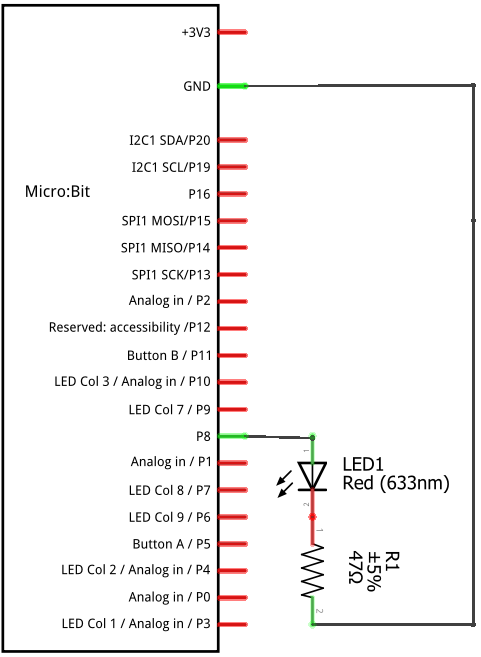
\includegraphics[width=0.75\textwidth]{figuren/externeLedCr}
			\caption{Een externe led aangesloten op P08 }
			\label{fig:exLd}
			
		\end{subfigure}
		\begin{subfigure}[b]{0.46\textwidth}
\begin{lstlisting}[caption={Het aansturen van een externe LED.},label={lst:extLd1}]
const int externeLed = 8;
			
void setup() {
	pinMode(externeLed, OUTPUT);  
}
				
void loop() {
  digitalWrite(externeLed,HIGH);
  delay(500);
  digitalWrite(externeLed,LOW);
  delay(500); 
}
\end{lstlisting}
		\end{subfigure}
		\captionsetup{justification=centering}
		\caption{Het aansturen van een externe LED. }
		\label{fig:vbExtld}
	\end{center}	
\end{figure}
De externe LED is aangesloten op poortnummer 8.
\begin{enumerate}
	\item In de \textcolor{arduinoGreen}{setup}() wordt dit poortnummer op output gezet,\\  (\textcolor{arduinoOrange}	{pinMode} (externeLed,  \textcolor{arduinoBlue}{OUTPUT})); 
\item In de \textcolor{arduinoGreen}{loop}() wordt:
\begin{enumerate}
	\item Een spanning gezet op poort 8 (\textcolor{arduinoOrange}{digitalWrite}(externeLed, \textcolor{arduinoBlue}{HIGH});) waardoor een elektrische stroom door de LED gaat lopen en deze licht gaat geven. 
	\item Hierna wordt een halve seconde gewacht.
	\item Daarna wordt op poort 8,  0 Volt gezet (\textcolor{arduinoOrange}{digitalWrite}(externeLed, \textcolor{arduinoBlue}{LOW});) en gaat de LED uit (er loopt geen elektrische stroom meer door de LED).
		\item Hierna wordt een halve seconde gewacht.
\end{enumerate} 
\end{enumerate}
 
\paragraph{De LED bij het blink programma in Listing \ref{lst:blink}:} is een onderdeel van een matrix, zoals in figuur \ref{fig:ledmtx2} wordt weergegeven.

\begin{minipage}{\linewidth}
	\begin{wrapfigure}[25]{r}{0.6\textwidth}
		\vspace{-15pt}
		\begin{center}
			\centering
			\captionsetup{justification=centering}
			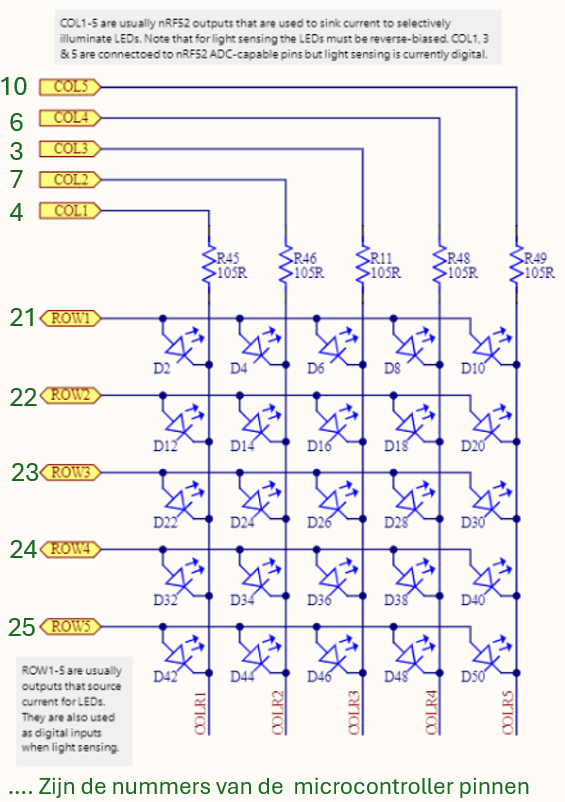
\includegraphics[width=0.45\textwidth]{figuren/LedMatrixV2Mnr}
		\end{center}
		%	\vspace{-14pt}
		\caption{Aansluitingen van de LED matrix..}
		\label{fig:ledmtx2}
	\end{wrapfigure}
	
~\vspace{5mm}\\
	Om de LED  (\img{figuren/diodeIc.png}) D2 aan te zetten, zou een elektrische stroom moeten lopen van  pin  \textcolor {Green}{21} door LED D2 naar pin \textcolor{Green}{4}.
	Dit kan voor elkaar verkregen worden door als eerst beide pinnen op output te zetten:\\
	\lstinline|	pinMode(4, OUTPUT);|\\ \lstinline|	pinMode(21, OUTPUT);|\\
	Vervolgens wordt pin \textcolor {Green}{4} laag gemaakt:\\
	 \lstinline|digitalWrite(4,LOW);|\\ en pin \textcolor {Green}{21} hoog gemaakt\\ \lstinline|digitalWrite(21,HIGH);|.\\
	 Indien pin \textcolor {Green}{21}  na een tijdje\\ \lstinline|delay(500);| weer laag wordt gemaakt\\ \lstinline|digitalWrite(21,LOW);| zal de LED uitgaan.
\end{minipage}


\section{Uitbreiding van de code.}

\begin{enumerate}
	
\item In het programma \textit{blink} van listing \ref{lst:blink} knippert de LED met een frequentie van 1 Hz ($\frac{1}{2}$ seconde aan en $\frac{1}{2}$ seconde uit).\\
\begin{enumerate}
	\item Wijzig in de schets de eerste \textcolor{BurntOrange}{delay}(500) (regel 17) naar \textcolor{BurntOrange}{delay}(100).
	\item   Klik op \img{figuren/ardIcUpl.png} of druk \colorbox{mygray}{\textbf{Ctrl + U}} om het programma te compileren en naar de Microbit te sturen.
\end{enumerate}

Je ziet nu dat de ‘aan’ tijd langer is.
\item Laat nu ook LED D6 mee Knipperen (LED D2 en D6 knipperen).
\item Laat nu ook LED D12 mee knipperen (LED D2, D6 en D12 Knipperen)
\item Laad nu ook LED D14 mee knipperen. (LED D2, D6, D12 en D14 Knipperen).\\ \texttt{Verklaar wat er gebeurt}

\end{enumerate}

\subsubsection{De matrix programmeren met behulp van de Adafruit library}



\subsubsection{Uitleg: Gebruik van de seriële poort}

 dit voorbeeld wordt de seriële poort gebruikt.

Je kunt de seriële poort gebruiken om te ‘debuggen’, oftewel controleren of je programma doet wat je er van verwacht. In The Challenge kun je het gebruiken om sensordata naar je PC te sturen.

Open de seriële monitor(Tools$\rightarrow$Serial Monitor) of (druk \colorbox{mygray}{\textbf{Ctrl + Shift + M}}) of klik op \img{figuren/ardIcMo.png}

Het programma drukt telkens ‘blink!’ af.\\ 
Zet “Show Timestamp” aan om de regels van elkaar te kunnen onderscheiden.\\ 
Zorg dat de ingestelde snelheid overeen komt met de instelling \textcolor{BurntOrange}{Serial.begin}(9600) in  \textcolor{OliveGreen}{setup}(). 
\begin{figure}[h!]
	\captionsetup{justification=centering}
	\includegraphics[width=0.99 \linewidth]{figuren/ardSerIns}
	\centering
	\caption{Instellingen van de seriële monitor.}
	\label{fig:arSeIn}
\end{figure}
De instellingen van de monitor kan gedaan worden in de statusbalk, zoals te zien is in figuur \ref{fig:arSeIn}.
Vaak wordt 9600 Baud (bits per seconde) gebruikt. Dit is gedaan omdat hiermee de data praktisch altijd stabiel verzonden wordt.

\subsection{Commando's verklaren.}

Geef in je eigen woorden weer wat de volgende commando’s doen (zoek uit via  \colorbox{mygray}{\textbf{Ctrl + Shift + F}})
\textcolor{BurntOrange}{pinMode}(LED, \textcolor{BlueGreen}{OUTPUT});\\
\vspace{1cm}
\hrule
~\\    
%\hrule
\vspace{1cm}
\textcolor{BurntOrange}{digitalWrite}(LED, \textcolor{BlueGreen}{LOW});\\
\vspace{1cm}
\hrule
~\\    
%\hrule
\vspace{0.8cm}
\textcolor{BurntOrange}{delay}(500);
 \vspace{1cm}
 \hrule
 ~\\    
 Wat denk je dat het grootste nadeel van \textcolor{BurntOrange}{delay}();  is?
 \vspace{1cm}
 \hrule
 
 \subsection{Dimmen van een led}
 
 We hebben al gezien dat je een pin als uitgang in kunt stellen en deze aan en uit kunt zetten.
 
 We gaan dezelfde pin nu op een andere manier gebruiken. We gaan de LED nu geleidelijk feller en minder fel laten branden, het Engelse werkwoord hiervoor is ‘to fade’. 
  \begin{enumerate}
 	\item  We gaan hierbij uit van de code uit de blinkdemo van listing \ref{lst:blink}.  Het knipperen van de LED wordt
 	in de \textcolor{arduinoGreen}{loop} gedaan, zoals in listing \ref{lst:blinkAfk} te zien is.
% 	\begin{lstlisting}[style=myArduino, caption= Het knipperen van de LED.,label={lst:blinkAfk},firstnumber=15]
  	\begin{lstlisting}[caption= Het knipperen van de LED.,label={lst:blinkAfk},firstnumber=15]		
 		void loop() {
 			
 			digitalWrite(LED, HIGH);
 			delay(500);
 			digitalWrite(LED, LOW);
 			delay(500);
 		}
 	\end{lstlisting} 
 	Hierbij wordt met het statement \textcolor{arduinoOrange}{digitalWrite}(LED, \textcolor{arduinoBlue}{HIGH}); de LED aangezet en met het statement \textcolor{arduinoOrange}{digitalWrite}(LED, \textcolor{arduinoBlue}{LOW}); de LED uitgezet.  In plaats van \textcolor{arduinoOrange}{digitalWrite} kan in sommige gevallen ook \textcolor{arduinoOrange}{analogWrite} gebruikt worden. Hiermee kan opgegeven worden hoeveel licht de LED geeft.
 	
 	Sla de blink op onder een andere naam, bijvoorbeeld Microbit-Fade. Verander de statement  \textcolor{arduinoOrange}{digitalWrite}(LED, \textcolor{arduinoBlue}{HIGH}); in \textcolor{arduinoOrange}{analogWrite}(LED, 10);
 	Klik vervolgens op \img{figuren/ardIcUpl.png} of druk \colorbox{mygray}{\textbf{Ctrl + U}} om het programma te compileren en naar de Microbit te sturen. Verklaar wat er gebeurd.
 	
 	Verander de 10 in een ander getal b.v. 70 en verklaar wat er gebeurd. De maximale waarde waarop de LED ingesteld kan worden is 255. Dit heeft te maken met het feit dat de waarde maar 8 bits groot is en 2$^{8}$ - 1 = 255.
 	%en het ingebouwde voorbeeld Fade van Arduino: Open Bestand $\rightarrow$ Voorbeelden $\rightarrow$ 01.Basics $\rightarrow$ Fade
 
 	\item  Pas het programma verder aan, zodat de LED steeds meer licht gaat geven. Indien de hoeveelheid licht die de LED geeft maximaal is, gaat de LED weer minder licht geven totdat de LED geen licht meer geeft, hierna gaat de LED weer meer licht geven, enz. Zoals weergegeven in het volgende filmpje\\  
 	\href{https://www.youtube.com/watch?v=J-VdHiCPVbQ/fade.mp4}{https://www.youtube.com/watch?v=J-VdHiCPVbQ/fade.mp4} te zien is.\\
 	\textbf{Lever deze opgave in op blackboard.}
   
  \end{enumerate}
 
 
 
\begin{comment}



 Gebruik de mogelijkheden van Arduino (en niet Google) om onderstaande vragen te beantwoorden, denk aan \colorbox{mygray}{\textbf{Ctrl + Shift + F}} en de commentaren die al in de code staan:
 Welke regel (welk commando) zorgt voor dit Fade effect? 


 \vspace{1cm}
 \hrule
 \vspace{1cm}
 Het mechanisme dat hier gebruikt wordt heet PWM. Waar staat de afkorting voor en wat doet het?
 \vspace{1cm}
 \hrule
 ~\\    
 \hrule
 \vspace{0.5cm}
\end{comment}
 Het mechanisme dat hier gebruikt wordt om de LED te dimmen heet PWM.\\
{ \texttt{\textit{Met PWM kun je niet alleen een led minder fel laten branden, maar zo kun je ook de snelheid van een motor regelen. De piepjes die je hoort bij een optrekkende tram of trein worden veroorzaakt door PWM aansturing.}}}
% \end{comment}
 
 \subsection{Het ontvangen van informatie vanaf de arduino-monitor en de beide knoppen.}
 
 Behalve dat de microbit data naar de monitor kan verzenden, kan deze ook data van de  monitor lezen.
 Dit kan gedaan worden door de data in het bovenste vierkant (zoals in figuur \ref{fig:ardMonRd} wordt weergegeven) in te typen en vervolgens op \textbf{Send} te klikken.
 \begin{figure}[h!]
 	\captionsetup{justification=centering}
 	\includegraphics[width=0.6 \linewidth]{figuren/arduinoMonRd}
 	\centering
 	\caption{Inputveld van de arduino monitor.}
 	\label{fig:ardMonRd}
 \end{figure}
Om in je programma de data te lezen, zal eerst gecheckt moeten worden of er al data via de seriële poort binnen gekomen is, dit kan gedaan worden met het statement:  \texttt{if(\textcolor{BurntOrange}{Serial.available}() \textgreater 0) \{ \}} daarna kan de data pas gelezen worden. 
Dit wordt gedaan met het statement:   \texttt{int getal=\textcolor{BurntOrange}{ Serial.read}();}, zoals te zien is in listing \ref{lst:serInp}.

%\begin{lstlisting}[style=myArduino,numbers=none ,caption= inlezen via de seriele poort.,label={lst:serInp}]
\begin{lstlisting}[numbers=none ,caption= inlezen via de seriele poort.,label={lst:serInp}]	
int getal=0;

void setup() {  
	Serial.begin(9600);
	Serial.println("Hoi embedded programmeurs!");
	
}

void loop(){
	if (Serial.available() > 0) {  //is er een character ingevoerd?
		getal= Serial.read();
		Serial.println(getal);
	}
}
\end{lstlisting} 
 Opdracht:
 
  \begin{enumerate}
 	\item Voer de code van Listing \ref{lst:serInp} uit en type in het invoerveld van de monitor de cijfers 012345 in, gevolgd door een enter.
 	Als het goed is verschijnt Figuur \ref{lst:serInp}
 
 \begin{figure}[h!]
 	\captionsetup{justification=centering}
 	\includegraphics[width=0.6 \linewidth]{figuren/ardMonChar.jpg}
 	\centering
	\caption{Uitvoering van listing \ref{lst:serInp}}
 		\label{fig:ardMonChr}
 \end{figure}
Wat opvalt is dat in plaats van het getal 012345 de getallen 48, 49, 50, 51, 52 en 53 worden uitgeprint. Dit heeft te maken dat het statement 
\texttt{int getal=\textcolor{BurntOrange}{ Serial.read}();} een character inleest, waarbij elke character een waarde heeft volgens de \href{https://nl.wikipedia.org/wiki/ASCII_(tekenset)}{ASCII} tabel.\\
Let op: Indien de monitor anders ingesteld staat dan "\texttt{\textit{No line ending}}", worden de onzichtbare characters (line feed en/of carriage return ) getoond. 
\item Pas het programma van listing 1 zodanig aan, zodat na invoering van je studentnummer en gebruik van het statement \texttt{int getal=\textcolor{BurntOrange}{ Serial.read}();} ook daadwerkelijk je studentnummer als een integer uitprint kan worden. 
 \begin{figure}[h!]
	\captionsetup{justification=centering}
	\includegraphics[width=0.8 \linewidth]{figuren/nummerloop}
	\centering
	\caption{diagram om  losse cijfers om te zetten naar een int. }
	\label{fig:progFig}
\end{figure}
Een schematische weergave van de oplossing, wordt in Figuur \ref{fig:progFig} weergegeven.
\small{Tip: kijk naar de sheets over het \textbf{decimale talstelsel met grondtal 10}}.\\
\textbf{Lever deze opgave in op blackboard.}
\end{enumerate}

\section{De (externe) pinnen van de microbit}
 
De Microbit heeft 21 pinnen (aansluitingen) die voor allerlei toepassingen bruikbaar zijn. In figuur \ref{fig:ardPinB} zijn de externe aansluitingen van de microbit te zien. 
\begin{figure}[h!]
	\captionsetup{justification=centering}
	\includegraphics[width=0.6 \linewidth]{figuren/microbitCon.jpg}
	\centering
	\caption{Pinlayout van de microbit.}
	\label{fig:ardPinB}
\end{figure}
Hierbij wordt aangegeven welke onderdelen van de microbit ook extern zijn te gebruiken. Bij de pinnen waarbij \fcolorbox{black}{Apricot}{ANALOG IN} staat, kan een externe analoge signaal van b.v. een externe sensor aangesloten worden. De pinnen genaamd \fcolorbox{black}{NavyBlue}{\textcolor{White}{P..}} zijn de pinnummers. In de Arduino IDE kan je die P weglaten en hoef je alleen het nummer op te geven, 0 t/m 20. Uitgebreidere informatie over de pinnen is te vinden op de website \href{https://tech.microbit.org/hardware/edgeconnector/}{tech.microbit.org/hardware/edgeconnector/}.\\
%\newpage

\subsection{Het lezen van externe signalen met de microbit.}

Stel op PIN P0 willen we een externe analoge sensor aansluiten. Voor de spanningswaarde die de sensor levert willen we een digitale waarde weten. 
Dit kan in de Arduino omgeving gedaan worden me het statement:\\

int sensorwaarde = \textcolor{arduinoOrange}{analogRead}(A0);

\begin{enumerate}
%	\item  Open \textbf{Bestand $\rightarrow$ Voorbeelden $\rightarrow$ 01.Basics $\rightarrow$ AnalogReadSerial}.
\item In programma listing \ref{lst:analogInp} wordt het analoge signaal van de externe PIN P0 gelezen.
%\begin{lstlisting}[style=myArduino,numbers=none ,caption= inlezen via een analoog signaal.,label={lst:analogInp}]
\begin{lstlisting}[numbers=none ,caption= inlezen via een analoog signaal.,label={lst:analogInp}]
	void setup() {  
		pinMode(0, INPUT); 
		Serial.begin(9600);
		Serial.println("Hoi embedded programmeurs!");
	}
	
	void loop(){
          // lees de analoge waarde op pin 0:
        int sensorValue = analogRead(A0);
        
        // print de ingelezen analoge waarde
        Serial.println(sensorValue);
        delay(100);        // delay 
	}

\end{lstlisting}
\begin{enumerate}
	\item  Maak een nieuw Arduino sketch aan en zet listing \ref{lst:analogInp} erin, Klik vervolgens op \img{figuren/ardIcUpl.png} of druk \colorbox{mygray}{\textbf{Ctrl + U}} om het programma te compileren en naar de Microbit te sturen. 
\item Zoek PIN 0 in Figuur \ref{fig:ardPinB}.
\item Leg je Microbit op tafel, raak hem niet aan. 
\item De Arduino omgeving heeft behalve een Seriële monitor ook een Seriële Plotter. Helaas kan maar één van beide monitor of plotter gebruikt worden. 
Indien de Seriële monitor open is, sluit deze dan en open de Seriële Plotter ( Tools $\rightarrow$ Serial Plotter of \colorbox{mygray}{\textbf{Ctrl + shift + L}}).
Raak met je vinger het gouden vlakje van pin 0 aan en kijk in de Seriële Plotter wat er gebeurt.
\item Tussen welke waardes op de linker as liggen de meetwaardes? \hrulefill \\	
 \footnotesize{\texttt{\textit{(Bij mij kwam deze uit tussen de 1000 zonder aanraken en de 750 )}} }
	
\end{enumerate}


\item Verander he statement  \textcolor{arduinoOrange}{analogRead}(A0); in \textcolor{arduinoOrange}{digitalRead}(A0); Klik vervolgens op \img{figuren/ardIcUpl.png} of druk \colorbox{mygray}{\textbf{Ctrl + U}} om het programma te compileren en naar de Microbit te sturen. Raak met je vinger het gouden vlakje van pin 0 aan en kijk in de Seriële Plotter wat er gebeurt. 

\item Bij het inlezen van een digitaal signaal is het niet wenselijk dat bij het aanraken van een draadje of een gouden vlakje de ingangswaarde instabiel wordt. Om dit te voorkomen kan bij Arduino de  \textcolor{arduinoBlue}{INPUT\_PULLUP} aangezet worden. Dit wordt gedaan met het statement: \textcolor{arduinoOrange}{pinMode}(0,\textcolor{arduinoBlue}{INPUT\_PULLUP}); 

\begin{minipage}{\linewidth}
\begin{wrapfigure}[25]{r}{0.54\textwidth}
	\vspace{-15pt}
	\begin{center}
		\centering
		\captionsetup{justification=centering}
		\includegraphics[width=0.32\textwidth]{figuren/microBitDraad}
	\end{center}
%	\vspace{-14pt}
	\caption{Input verbonden met de GND .}
	\label{fig:micrDraad}
\end{wrapfigure}
Zet de \textcolor{arduinoBlue}{INPUT\_PULLUP} aan door het statement 
\textcolor{arduinoOrange}{pinMode}(0,\textcolor{arduinoBlue}{INPUT\_PULLUP});  
te plaatsen in de \textcolor{arduinoGreen}{setup} en bekijk wat het resultaat is bij het inlezen van de digitale en analoge waarden. Indien je een draadje bij de hand heb, verbindt de GND met PIN 0, zoals te zien is in figuur \ref{fig:micrDraad}, het gevolg van de PULL\_UP zal zijn dat alleen nog de waarde 0 ingelezen wordt indien de pin ook daadwerkelijk verbonden wordt met de GND.
\end{minipage}



\begin{comment}
Zet de \textcolor{arduinoBlue}{INPUT\_PULLUP}  aan door het statement  \textcolor{arduinoOrange}{pinMode}(0,\textcolor{arduinoBlue}{INPUT\_PULLUP});  
te plaatsen in de \textcolor{arduinoGreen}{setup} en bekijk wat het resultaat is bij het inlezen van de digitale en analoge waarden.
\end{comment}
\end{enumerate}
\begin{comment}
Wat zie je gebeuren? 
\vspace{1cm}
\hrule
\vspace{0.8cm}
Tussen welke waardes op de linker as liggen de meetwaardes? \hrulefill

Hoeveel bits zijn nodig om dit getal (de hoogste waarde) weer te geven?  \hrulefill

Voeg nu deze regel toe in het \textcolor{OliveGreen}{setup}() deel:

\hspace{1cm}
\textcolor{BurntOrange}{pinMode}(0,\textcolor{BlueGreen}{INPUT\_PULLUP});\\

Sla je programma op met \colorbox{mygray}{\textbf{Ctrl + S}} en upload het programma met \colorbox{mygray}{\textbf{Ctrl + U}} , open de Seriële Plotter.

Wat zie je nu gebeuren?
\vspace{1cm}
\hrule
Tussen welke waardes op de linker as liggen de meetwaardes? \hrulefill
\end{comment}
%\newpage
\begin{minipage}{\linewidth}
\footnotesize{\texttt{\textit{Zoals je ziet is de ingang ongevoelig als je \textcolor{arduinoBlue}{INPUT\_PULLUP} aanzet. Je gebruikt \textcolor{arduinoBlue}{INPUT\_PULLUP} als je een ingang naar een stabiele ‘hoog’ toestand wilt hebben. Je gebruikt deze modus samen met digitalRead() als je een schakelaar wilt uitlezen. Als je de schakelaar indrukt wordt de pin laag.\\
De knopjes op de Microbit gebruiken een \textbf{externe} pull-up weerstand, met \textcolor{arduinoBlue}{INPUT\_PULLUP} zet je een pull-up weerstand in de microcontroller aan.\\ Kijk eens online voor meer uitleg over de principes van een  \href{https://www.freecodecamp.org/news/a-simple-explanation-of-pull-down-and-pull-up-resistors-660b308f116a/}{pull\_up weerstand}.\\ \\
Voor verdere uitleg zie \href{https://www.arduino.cc/en/Tutorial/DigitalPins}{www.arduino.cc/en/Tutorial/DigitalPins}
}}}
\end{minipage}
\normalsize
\subsection{Een denderende schakelaar.}

Behalve dat bij het inlezen van de waarde van een externe schakelaar regelmatig een pull\_up weerstand noodzakelijk is. 
Treedt er nog een ander probleem op, namelijk een schakelaar die dendert ook wel bouncing genaamd.

Indien een schakelaar wordt ingedrukt sluit deze bijna nooit in 1 keer, maar veert een aantal keren op en neer. Dit fenomeen wordt weergegeven in Figuur \ref{fig:swDend}, 
\begin{figure}[h!]
	\captionsetup{justification=centering}
	\includegraphics[width=0.6 \linewidth]{figuren/denderen}
	\centering
	\caption{Een denderende schakelaar\cite{williams2014make}.}
	\label{fig:swDend}
\end{figure}
waar te zien is dat bij het indrukken en loslaten van het knopje de schakelaar 'stuitert'. 
Één van de eenvoudigste manieren om dit op te lossen is door even te wachten (een paar milliseconden) en vervolgens te controleren of de knop nog steeds is ingedrukt. Dit wordt weergegeven in listing \ref{lst:denderBut}
%\begin{lstlisting}[style=myArduino, caption= Omgaan met een denderende schakelaar.,label={lst:denderBut}]
\newpage
\begin{lstlisting}[caption= Omgaan met een denderende schakelaar.,label={lst:denderBut}]
const int knopA = 5;     // Knop A is aangesloten op poortnummer 5
const int knopB = 11;    // Knop B is aangesloten op poortnummer 11

void setup() {  
	Serial.begin(9600);
	Serial.println("microbit is ready!");
	
	pinMode(knopA, INPUT);  
	pinMode(knopB, INPUT);   
}
boolean isKnopIngedrukt(int); //declaratie van de funcie

void loop(){
	
	if( isKnopIngedrukt(knopA) )
	Serial.println("A is ingedrukt");
	
	if( isKnopIngedrukt(knopB) )
	Serial.println("B is ingedrukt");       
	
	delay(10);
}

boolean isKnopIngedrukt( int knop) {
	if (! digitalRead(knop)) {  //Is de knop soms ingedrukt ?
		delay(2);      //wacht 2 milliseconde 
		if (! digitalRead(knop)) { //Is knop nog steeds ingedrukt
			return true;
		}
	}
	return false;
}
\end{lstlisting}

Hierbij wordt in de functie \texttt{\textit{\textcolor{arduinoBlue}{boolean} isKnopIngedrukt(\textcolor{arduinoBlue}{int});}} als eerste gekeken of de knop is ingedrukt, vervolgens wordt er 2 miliseconde gewacht, waarna opnieuw gekeken wordt of de knop is ingedrukt. Is dit zo dan wordt een \textcolor{arduinoBlue}{true} mee teruggegeven anders een \textcolor{arduinoBlue}{false}.

In listing \ref{lst:changeBut} is te zien dat er een detectie plaatsvindt wanneer de toestand van de schakelaar verandert.
\begin{lstlisting}[caption= Een toestandverandering van de schakelaar.,label={lst:changeBut}]

const int COL1 = 4; 
const int ROW1 = 21;
const int knopA = 5;     // Knop A is aangesloten op poortnummer 5
const int knopB = 11;    // Knop B is aangesloten op poortnummer 11

boolean isKnopIngedrukt(int);

int knopTeller = 0;  
boolean knopToestand = false;
boolean vorigeKnopToestand = false;
int ledStatus = LOW;

void setup() {  
	Serial.begin(9600);
	Serial.println("microbit is ready!");
	pinMode(COL1, OUTPUT);
	pinMode(ROW1, OUTPUT);
	pinMode(knopA, INPUT);  
	pinMode(knopB, INPUT);   
    digitalWrite(COL1, LOW);
}

void loop(){
	knopToestand = isKnopIngedrukt(knopA);
	if(knopToestand != vorigeKnopToestand)  //heeft er een verandering plaatsgevonden?
	if (knopToestand == true) {
		knopTeller++;
		ledStatus = !ledStatus;
		Serial.println(knopTeller);
	}
	delay(50);
	vorigeKnopToestand = knopToestand;
	digitalWrite(ROW1, ledStatus);
}

boolean isKnopIngedrukt( int knop) {
	if (! digitalRead(knop)) {  //Is de knop soms ingedrukt ?
		delay(2);      //wacht 2 milliseconde 
		if (! digitalRead(knop)) { //Is knop nog steeds ingedrukt
			return true;
		}
	}
	return false;
}

\end{lstlisting}

%Open Bestand $\rightarrow$ Voorbeelden $\rightarrow$ Microbit-HHS $\rightarrow$ 04B.StateChangeDetection en
Open het voorbeeldprogramma \texttt{\textit{veranderToestandDrukknop.ino}} (dit is listing \ref{lst:changeBut} )en upload het naar de Microbit.
Bestudeer de code en kijk hoe het programma werkt. Het is de bedoeling dat na elke druk op knopA de led aan of uit gaat (wisselt van toestand) en dat de teller steeds met 1 opgehoogd wordt. 
	\begin{enumerate}[label=(\Alph*)]

	\item In figuur \ref{fig:swToestand} wordt het signaal van de button weergegeven.
\begin{figure}[h!]
	\captionsetup{justification=centering}
	\includegraphics[width=0.8 \linewidth]{figuren/toestandButtonPin}
	\centering
	\caption{Weergaven van het signaal, indien de button wordt ingedrukt en weer wordt losgelaten.}
	\label{fig:swToestand}
\end{figure}
In welke toestand (1 t/m 4 )  bevindt zich de variabele \texttt{knopToestand} en \texttt{vorigeKnoptoestand} indien de toestand van de LED verandert en de teller met 1 verhoogd wordt?
\item Wat is het nut van het statement \textcolor{arduinoOrange}{delay}(50) op regel 31?\hrulefill
\item Wat is het resultaat indien de outputpin COL1 van listing \ref{lst:changeBut} op \textcolor{arduinoBlue}{HIGH} gezet wordt?	
\item Breid listing \ref{lst:changeBut} uit, zodat de teller met 1 verlaagd wordt indien met knopB een toestand verandering van 3 naar 4 plaatsvindt.\\
\textbf{Upload deze opgave op blackboard.}
	
\end{enumerate}



\section{Bitwise operaties.}
\label{chap:biw}

Zoals in hoofdstuk \ref{sec:matrix} staat vermeldt heeft de firma Adafruit voor het matrix display een speciale component gemaakt waardoor het matrix display eenvoudig te programmeren is. Listing \ref{lst:matrixaan} is hier een voorbeeld van.
\begin{lstlisting}[caption={Het aanzetten van een LED},label={lst:matrixaan}]
#include <Adafruit_Microbit.h>
#define LED0 0  //definieer LEDx tot een waarde
#define LED1 1
#define LED2 2
#define LED3 3
#define LED4 4

Adafruit_Microbit_Matrix matrixMbit; //maak een LED matrix aan.
const uint8_t
smile_bmp[] =
{ B00000,
	B01010,
	B00000,
	B10001,
	B01110, };
uint8_t matrixje[] =
{ B00000,
	B00000,
	B00000,
	B00000,
	B00000, };

void setup() {
	Serial.begin(9600);
	Serial.println("Welkom bij embedded!");
	
	matrixMbit.begin();
	matrixMbit.show(smile_bmp);
	delay(2000);
	matrixMbit.show(matrixje);
	delay(2000);  
	//zet rechterLED bovenste rij aan
	matrixje[0]= 1 << LED0; //schuif 1, LED0 plaatsen op naar links.
	matrixMbit.show(matrixje);
	delay(2000);  
	//zet linkerLED bovenste rij aan 
	matrixje[0] = 1 << LED4; //schuif 1, LED4 plaatsen op naar links.
	matrixMbit.show(matrixje);
}
void loop() {
}
\end{lstlisting}
Wat opvalt aan Listing \ref{lst:matrixaan} is dat er een hoop define's staan aan het begin. De bedoeling van deze define's is dat de code eenvoudiger te lezen is.
Indien in de code  \small{\texttt{\textit{1 \textless\textless  ~LED4}}} staat, weet de lezer gelijk dat de $4^{e}$ LED bedoeld wordt. Verder is te zien hoe een LED aangezet kan worden door de betreffende bit in een array van 8 bits data, een 1 te maken. Dit wordt gedaan door een 1 (0b00000001) een aantal plaatsen naar links op te laten schuiven. Zoals te zien is in onderstaand statement:\\
\texttt{\textit{matrixje[0]= 1 \textless\textless  ~LED0;}}\\
Hierbij staat de \texttt{1} voor het aantal plaatsen dat LED0 naar links wordt opgeschoven. LED0 staat gedefinieerd op regel 2 van Listing \ref{lst:matrixaan}
\begin{enumerate}
	\item Installeer \href{https://learn.adafruit.com/use-micro-bit-with-arduino/adafruit-libraries}{de Adafruit Libraries} indien dit nog niet gedaan is.
	\item
	\begin{enumerate}

	\item Open voorbeeldcode matrixSmpl (dit is Listing \ref{lst:matrixaan}). 
	\item Breid het programma zodanig zodat uit, zodat zowel LED0 als LED4 van de 2e rij aangaan. Maak hierbij gebruik van de operatoren '\textless\textless' en '\textbar'(bitwise or). Doe dit zoals in de theorie besproken is.
	
%	\begin{table}[h!]
\setlength\arrayrulewidth{2pt}
		\begin{tabular}{|c|c|c|}
			\hline
%			\colorbox{yellow}{\textbf{A}} &\colorbox{yellow}{\textbf{B} & \colorbox{Yellow}{\textbf{AB}}   \\ \hline
          \rowcolor{yellow}
		    A  & B     & A \textbar~ B       \\ \hline          
		    0  & 0     & 0       \\ \hline
			0      & 1     & 1       \\ \hline
			1     & 0     & 1       \\ \hline
			1    & 1     & 1       \\ \hline
		\end{tabular}\\
De bitwise OR 
%	\end{table}
	
	\item Breid het programma uit zodat 2 seconde nadat beide LEDS uit B aangegaan zijn, de linker boven LED (LED4) weer uitgaat. Maak hierbij gebruik van de operatoren '\textless\textless' ,  '\&' en  ' $\sim$'. Doe dit zoals in de theorie besproken is.
	
	\setlength\arrayrulewidth{2pt}
	\begin{tabular}{|c|c|c|}
		\hline
		%			\colorbox{yellow}{\textbf{A}} &\colorbox{yellow}{\textbf{B} & \colorbox{Yellow}{\textbf{AB}}   \\ \hline
		\rowcolor{yellow}
		A  & B     & A \& B       \\ \hline          
		0  & 0     & 0       \\ \hline
		0      & 1     & 0       \\ \hline
		1     & 0     & 0       \\ \hline
		1    & 1     & 1       \\ \hline
	\end{tabular}\\
	De bitwise AND 
	\item Door met bitwise operaties te werken, kan op een eenvoudige wijze een LED dat aan is, uitgezet worden en een LED dat uit is aangezet worden. Dit kan gedaan worden met de exclusief OR operator, zoals te zien is in onderstaand tabel. 
	Breid het programma uit zodat 2 LEDS van de onderste rij aan en uitgaan door de exclusief OR functie te gebruiken. Maak hierbij onder ander gebruik van de operator \^ ~. Do dit zoals in de theorie besproken is.
	
	\setlength\arrayrulewidth{2pt}
	\begin{tabular}{|c|c|c|}
		\hline
		%			\colorbox{yellow}{\textbf{A}} &\colorbox{yellow}{\textbf{B} & \colorbox{Yellow}{\textbf{AB}}   \\ \hline
		\rowcolor{yellow}
		A  & B     & A \^ ~ B       \\ \hline          
		0  & 0     & 0       \\ \hline
		0      & 1     & 1       \\ \hline
		1     & 0     & 1      \\ \hline
		1    & 1     & 0       \\ \hline
	\end{tabular}\\
	De bitwise XOR 
	
	\item Er kan ook getest worden of een LED aan is met behulp van bitwise operatoren.\\	\textcolor{cyan}{uint8\_t} hulpje= matrixje[0];\\
	\textcolor{OliveGreen}{if}(hulpje ...  .....) \{ \\
\}.

Vul het \textcolor{arduinoGreen}{if} statement in en toon aan dat een LED aan of uit is.
 \end{enumerate}

\item In het volgende voorbeeld gaat steeds een LED van rechts naar links aan.

\begin{lstlisting}[caption={Looplicht van de bovenste rij.},label={lst:matrixaan2}]
#include <Adafruit_Microbit.h>

Adafruit_Microbit_Matrix matrixMbit; //maak een LED matrix aan.

uint8_t matrixje[] =
{ B00000,
	B00000,
	B00000,
	B00000,
	B00000, };

void setup() {
	Serial.begin(9600);
	Serial.println("Welkom bij embedded!");

    matrixMbit.begin();
	matrixMbit.show(matrixje);
	delay(1000);  
}

uint8_t nr=0;
uint8_t hulpje;

void loop() {
	hulpje = 1 << nr; //schuif 1, nr plaatsen op naar links.
	matrixje[0]=hulpje; //De bovenste rij van de matrix krijgt de 
	matrixMbit.show(matrixje);
	delay(1000);
	nr++;
	if (nr == 5) {
	    nr=0;
	}        
}
\end{lstlisting}
Op regel 5 wordt een matrix component aangemaakt. Het tonen van de matrix wordt met de show functie gedaan (regel 16 en en 26).

\begin{enumerate}
	\item Download de  \href{https://github.com/JohnVi-hhs/embsysP/tree/main/voorbeelden/matrixloopl.ino}{voorbeeldcode van GitHub} of van brightspace of kopieer listing \ref{lst:matrixaan} in een nieuwe Arduino schets en voer deze uit.\\
	Probeer de uitvoer te verklaren.

\item Maak een functie \texttt{void \textit{zetLedAan}(unint8\_t rij,uint8\_t kolom);} die de LED op kolom en rij aanzet. Maak hierbij gebruik van de bitwise operator \textbar ~ zoals besproken tijdens de les.
\item Maak een functie \texttt{void \textit{zetLedUit}(unint8\_t rij,uint8\_t kolom);} die de LED op kolom en rij uitzet. Maak hierbij gebruik van de bitwise operatoren \& en $\sim$ zoals besproken tijdens de les.
\item Maak een functie \texttt{bool \textit{isLedAan}(unint8\_t rij,uint8\_t kolom);} die checkt of de LED op kolom en rij aan is. Maak hierbij gebruik van een bitmasker zoals besproken tijdens de les.

	\item Pas listing \ref{lst:matrixaan} met behulp van de bovenstaande functies zodanig aan, zodat:
\begin{enumerate}%[label=\arabic*.]
	\item Nadat de eerste rij geweest is, bij de tweede rij de ledjes \'{e}\'{e}n voor \'{e}\'{e}n  aangaan. 
	\item Na de tweede rij bij de derde rij de ledjes \'{e}\'{e}n voor \'{e}\'{e}n  aan gaan. 
	\item Na de laatste rij bij de eerste rij de ledjes \'{e}\'{e}n voor \'{e}\'{e}n  aan gaan. 
\end{enumerate}

\textbf{Upload het resultaat op blackboard.}
\end{enumerate}\label{opdr:loppl}
\item Maak een looplicht dat gaat over alle 5 de rijen van de matrix zoals figuur \ref{fig:loopl} laat zien.

\begin{figure}[H]
	\captionsetup{justification=centering}
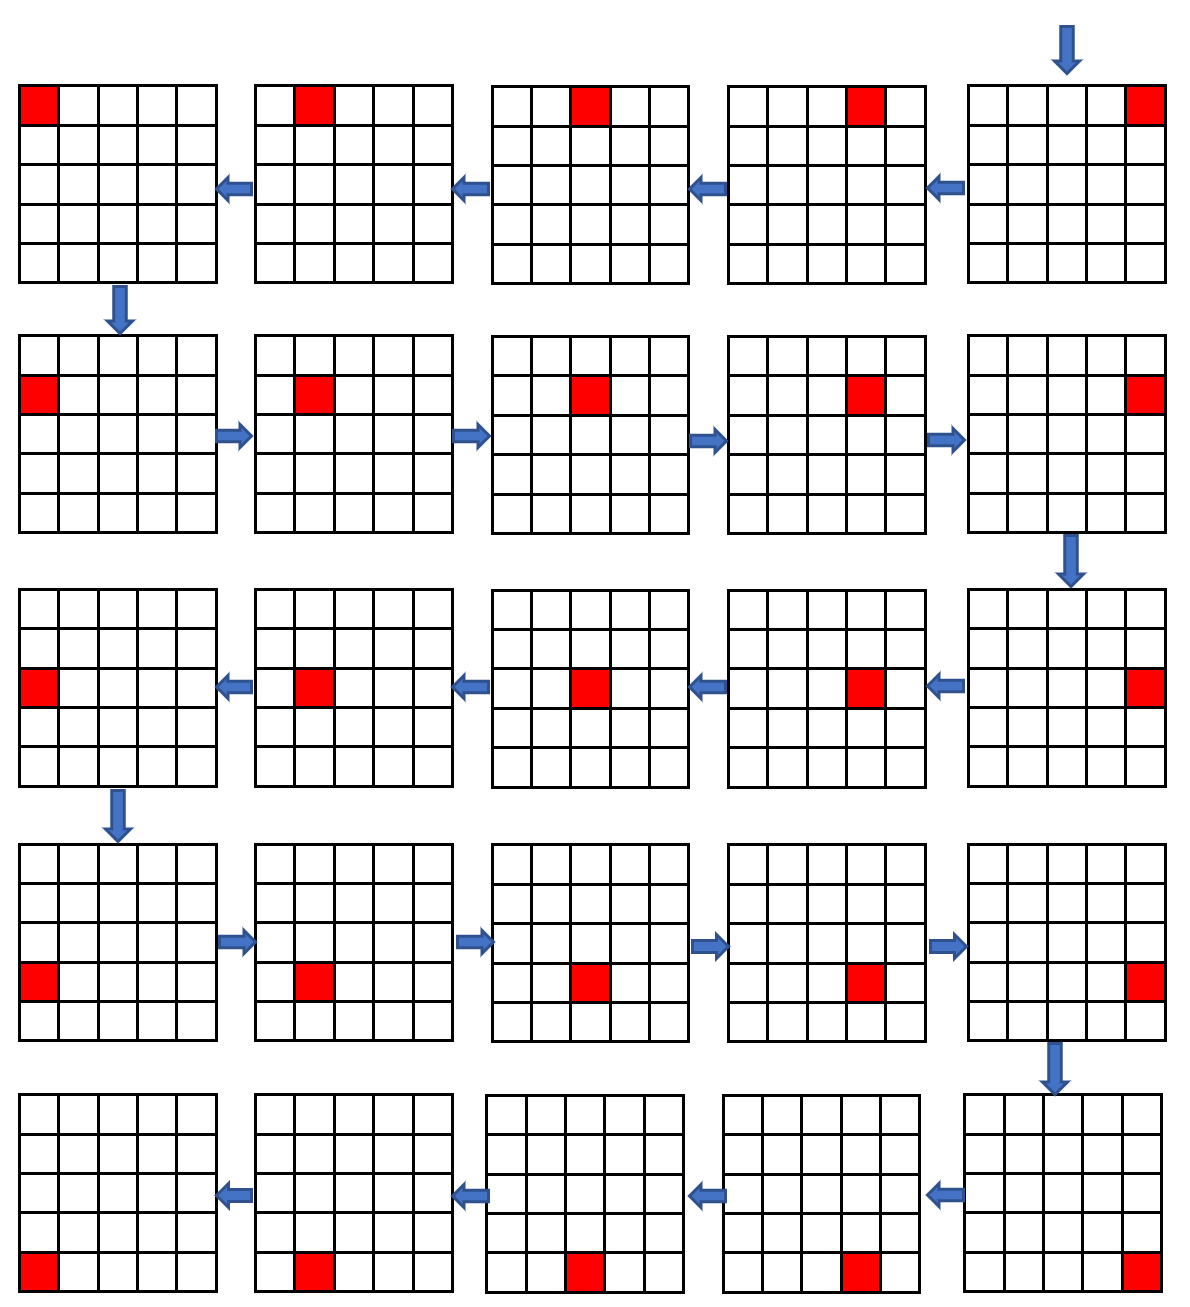
\includegraphics[width=0.6 \linewidth]{figuren/looplicht}
\centering
\caption{De volgorde van het looplicht.}
\label{fig:loopl}
\end{figure}

Begin rechtsboven (bit 0 van de ${0^{e}}$ rij in de matrix) en zet vervolgens steeds de LED links aan. Doe dit tot laatste LED van de rij.
Ga 1 rij naar beneden en zet vervolgens de LED rechts van de rij aan. Doe dit tot en met het $1^{e}$ bit.
Ga 1 rij naar beneden en zet vervolgens de LED links van de rij aan. Doe dit tot en met de laatste LED en ga vervolgens een rij naar beneden.
Doe dit tot en met de laatste rij en begin vervolgens weer op de eerste rij, zoals in het volgende filmpje \href{https://www.youtube.com/shorts/8ZyYWEiXsm0} {
	looplicht}
	te zien is.\\
\textbf{Upload het resultaat op blackboard.}
\end{enumerate}

\paragraph{Challenge opdracht}\label{opdr:accSens}

Op de micro:bit zitten verschillende sensoren. Eén van de sensoren is een \href{https://youtu.be/9WAckt2vrrQ}{accelerometer sensor}.
Het programma in listing \ref{lst:acc} toont de x,y en z waarde van de accelerator sensor.
\begin{enumerate}

	\item Download  listing \ref{lst:acc} van \href{https://github.com/JohnVi-hhs/embsysP/tree/main/voorbeelden/accelerator.ino}{ GitHub} of van brightspace of kopieer listing \ref{lst:acc} in een nieuwe arduino omgeving en voer deze uit.
	\item Pas het programma zodanig aan, zodat de LED in de richting beweegt, waarin micro:kit gehouden wordt.

	\end{enumerate}

\begin{lstlisting}[caption={Looplicht van de bovenste rij.},label={lst:acc}]
#include <LSM303AGR_ACC_Sensor.h>

#define DEV_I2C Wire1   // Wire1 is voor de interne I2C bus 
#define LED ROW1 


// Nodig voor de accelerator 
LSM303AGR_ACC_Sensor Acc(&DEV_I2C);


const int COL1 = 4;   
const int ROW1 = 21;   

void setup() {
	// Led.
	
	pinMode(COL1, OUTPUT);
	digitalWrite(COL1, LOW);
	pinMode(ROW1, OUTPUT);
	
	// Initialisatie van de serieele.
	Serial.begin(9600);
	
	// Initialisate I2C bus (wordt veel gebruikt om sensors).
	DEV_I2C.begin();
	
	// Initialisatie van de accelarator.
	Acc.begin();
	Acc.Enable();
	
	uint8_t a;
	Acc.IO_Read(&a,0x0F,1);
	Serial.print("Ik ben: ");
	Serial.println(a);
}

void loop() {
	// Led blinking.
	digitalWrite(LED, HIGH);
	delay(250);
	digitalWrite(LED, LOW);
	delay(250);
	
	// Lees de accelerometer van de LSM303AGR uit.
	int32_t accelerometer[3];
	Acc.GetAxes(accelerometer);
	
	// Output data.
	Serial.print("| Acc[x/y/z] ");
	Serial.print(accelerometer[0]);
	Serial.print(" ");
	Serial.print(accelerometer[1]);
	Serial.print(" ");
	Serial.print(accelerometer[2]);
	Serial.println(" |");
}
\end{lstlisting}


%\chapter{De bewegingssensor  \normalsize{(week 3).}}
\label{chap:bewSen}

De bewegingssensor, welke in rood wordt aangegeven in figuur \ref{fig:motion}, bestaat uit twee hoofdonderdelen, een accelerometer en een kompas. We gaan eerst aan de slag met een voorbeeld dat de bewegingssensor demonstreert, vervolgens met de magnetometer. Waarna beide onderdelen in 1 programma worden bewerkt.
\begin{figure}[h!]
	\captionsetup{justification=centering}
	\includegraphics[width=0.2 \linewidth]{figuren/motion}
	\centering
	\caption{Plaats van de bewegingssensor.}
	\label{fig:motion}
\end{figure}

\begin{enumerate}
%	\item  Open Bestand $\rightarrow$ Voorbeelden $\rightarrow$ Microbit-HHS $\rightarrow$ Microbit\_Bewegingssensor\_demo.
\item Installeer de \textit{STM32duino LSM303AGR} library in de arduino. 
Ga naar Sketch $\rightarrow$Include Library $\rightarrow$Manage Libraries of \colorbox{mygray}{\textbf{Ctrl + shift + I}} en type in het zoekveld STM32duino LSM303 zoals te zien is in Figuur \ref{fig:stm32303}.
\begin{figure}[h!]
	\captionsetup{justification=centering}
	\includegraphics[width=0.6 \linewidth]{figuren/stm32duinoLib}
	\centering
	\caption{Installeren van de STM32duino LSM303AGR.}
	\label{fig:stm32303}
\end{figure}
\item Open het voorbeeldprogramma accelerator.
\item Compileer en upload het voorbeeld naar je Microbit.
\item Als het programma werkt, dan knippert de led linksboven. 
\end{enumerate}

\section{De accelerator}
Stel dat ik in The Challenge de Microbit wil gebruiken om te kijken of de deksel van een container ver genoeg opengaat, dan moet ik dat kunnen meten. De bewegingssensor is daar ideaal voor.
\begin{figure}[h!]
	\captionsetup{justification=centering}
	\includegraphics[width=0.35 \linewidth]{figuren/microbit_axes}
	\centering
	\caption{Registratie van de accelerator \cite{microbitAccel}.}
	\label{fig:accel}
\end{figure}
De accelerometer meet de versnelling (beweging) in zowel de X, Y en de Z richting, zoals in figuur \ref{fig:accel} te zien is.

\newpage
De listing van het programma wordt weergegeven in listing \ref{lst:linkaccel}
\begin{lstlisting}[caption={Uitlezen van de accelarator},label={lst:linkaccel}]
#include <LSM303AGR_ACC_Sensor.h>

#define DEV_I2C Wire1   // Wire1 is voor de interne I2C bus 

#define LED ROW1 

// Components.
LSM303AGR_ACC_Sensor Acc(&DEV_I2C);

const int COL1 = 4;   
const int ROW1 = 21;   

void setup() {
	
	pinMode(COL1, OUTPUT);  //aansturing linkerboven LED in matrix
	digitalWrite(COL1, LOW);
	pinMode(ROW1, OUTPUT);
	
	Serial.begin(9600);  	// Initialize serial for output.
	
	DEV_I2C.begin();   	// Initialize I2C bus.
	
	Acc.begin();  	// Initlialize accelarator.
	Acc.Enable();

	uint8_t a;
	Acc.IO_Read(&a,0x0F,1);  //lees waarde Who_am_I register.
	Serial.print("Ik ben: ");
	Serial.println(a);
}

void loop() {
	// Led blinking.
	digitalWrite(LED, HIGH);
	delay(250);
	digitalWrite(LED, LOW);
	delay(250);
	
	int32_t accelerometer[3];
	Acc.GetAxes(accelerometer); 	// Read accelerometer LSM303AGR.
	
	// Output data.
	Serial.print("| Acc[mg]: ");
	Serial.print(accelerometer[0]);
	Serial.print(" ");
	Serial.print(accelerometer[1]);
	Serial.print(" ");
	Serial.print(accelerometer[2]);
	Serial.println(" |");
}
\end{lstlisting}

Op regel 8 wordt een software accelerometer. aangemaakt, die in de \textcolor{OliveGreen}{setup}()  (regel 23 en 24) wordt geïnitialiseerd. In de \textcolor{OliveGreen}{loop}() worden de waarden van de accelerator-sensor opgehaald en in een array gezet (regel 40).  
De opgehaalde waarden worden in de regels 44, 46 en 48 uitgeprint.

Ga als volgt te werk:
\begin{enumerate}
\item Open nu de seriële plotter.
\item Kijk naar de seriële plotter en kantel de Microbit langzaam naar links en naar rechts totdat deze verticaal staat. Doe dat ook naar voor en achter. Draai hem om zijn as. Kijk welke waarde verandert.
\item Zoek een waarde die overeenkomt met de richting die je zoekt, zet de Microbit bijvoorbeeld op zijn rechter zijkant. Je ziet twee meetwaarden die duidelijk meebewegen. Beweeg de Microbit terwijl je hem op zijn zij hebt op en neer. 
%Eén van de twee lijnen geeft een flinke uitslag, de andere niet. Degene die heftig reageren zijn die van de accelerometer, die moet je hebben. Die van de magnetometer reageren ook, maar die zijn afhankelijk van de positie van je Microbit ten opzichte van het noorden (als een kompas). 

\item Bepaal nu (met de seriële monitor) ongeveer de waarde die deze lijn heeft bij een hoek van 45 graden. We maken een aanpassing in het programma zodat deze een melding geeft als de hoek groter is dan 45 graden. In dat geval zetten we de led linksboven aan.
\item \textbf{\underline{Opdracht:}} Zoek de waardes uit en laat de led aangaan boven de 45 graden en weer uitgaan onder de 45 graden. Makkie, toch? Beetje simpel. We gaan meerdere ledjes aansturen.

\item \textbf{\underline{Combineer dit met: Hoe kunnen we de leds (eenvoudig) aansturen?: }}

Open het voorbeeldprogramma \texttt{\textit{heenEnWeer.ino}}. Om dit programma te laten werken zal de 	\href{https://learn.adafruit.com/use-micro-bit-with-arduino/adafruit-libraries}{de Adafruit Libraries}
geïnstalleerd moeten worden. In hoofdstuk \ref{chap:biw} word hier dieper op ingegaan.
%Open Bestand $\rightarrow$ Voorbeelden $\rightarrow$ Microbit-HHS $\rightarrow$ 3B.ForLoopIteration-met-library
\item Compileer en upload het voorbeeld naar je Microbit.
\item Kijk hoe de aansturing van de LEDs werkt en kopieer de benodigde code uit het voorbeeldprogramma \texttt{\textit{heenEnWeer.ino}} naar de bewegingssensor demo. Zorg eerst dat één ledje gaat branden aan de kant waar je de Microbit naartoe kantelt (alsof je een knikker op een dienblad hebt). Breid dit dan uit naar 4 leds (voor, achter, links, rechts) en uiteindelijk naar 8 leds (de leds op de hoeken erbij). 

Als je dit op een echt slimme manier wilt doen, dan gebruik je geen ‘if’ statements maar bereken je de pixellocatie uit de accelerometer waarden. Gebruik dan wel ‘if’ om te clippen.\\
\textbf{Upload het programma op blackboard.}


\end{enumerate}

\section{Het kompas}

Voor het kompas, geldt in principe hetzelfde alleen moet er nu een software-magnetometer aangeroepen worden. Dit kan gedaan worden met het volgende statement:\\
\texttt{\textit{LSM303AGR\_MAG\_Sensor Mag(\&DEV\_I2C);}}\\
Vergeet niet de magnetosensor te includen.\\
\texttt{\textit{\#include \textless LSM303AGR\_MAG\_Sensor.h \textgreater}}

\paragraph{Opdracht:}
Pas Listing \ref{lst:linkaccel} zodanig aan, zodat behalve de accelerator ook de magnetometer wordt aangeroepen en de waarden worden uitgeprint op de monitor. 
\textbf{Upload het programma op blackboard.}


%%\subsection{Het gebruik van de LED matrix.}
\chapter{Het gebruik van de LED matrix \normalsize{(week 4)}.}
\label{chap:matrix}

Indien we een externe LED op de microbit aansluiten, zoals in figuur \ref{fig:schemaExLd} wordt weergegeven, kunnen we deze direct aansturen, zoals listing \ref{lst:extLd} laat zien.
\begin{figure}[h!]
	
	\centering
	\begin{center} 	
		\begin{subfigure}[b]{0.43\textwidth}
			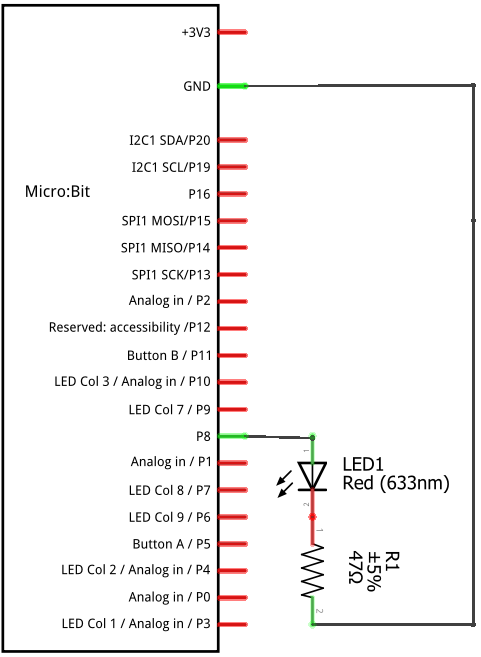
\includegraphics[width=0.85\textwidth]{figuren/externeLedCr}
			\caption{Een externe led aangesloten op P08 }
			\label{fig:schemaExLd}
			
		\end{subfigure}
		\begin{subfigure}[b]{0.46\textwidth}
\begin{lstlisting}[caption={Het aansturen van een externe LED.},label={lst:extLd}]
const int externeLed = 8;
				
   void setup() {

		pinMode(externeLed, OUTPUT);  
	}
				
	void loop() {
		digitalWrite(externeLed,HIGH);
		delay(500);
		digitalWrite(externeLed,LOW);
		delay(500); 
	}
\end{lstlisting}
		\end{subfigure}
		\captionsetup{justification=centering}
		\caption{Het aansturen van een externe LED. }
		\label{fig:exampleInh}
	\end{center}	
\end{figure}
De externe LED wordt aangesloten op poortnummer 8. In de \textcolor{arduinoGreen}{setup}() wordt dit poortnummer op output gezet. 
In de \textcolor{arduinoGreen}{loop}() wordt als eerste een spanning gezet op poort 8 (\textcolor{arduinoOrange}{digitalWrite}(externeLed, \textcolor{arduinoBlue}{HIGH});) waardoor een elektrische stroom door de LED gaat lopen en deze licht gaat geven. 
Hierna wordt een halve seconde gewacht, daarna wordt op poort 8,  0 Volt gezet (\textcolor{arduinoOrange}{digitalWrite}(externeLed, \textcolor{arduinoBlue}{LOW});) en gaat de LED uit (er loopt geen elektrische stroom meer door de LED).
Kijken we naar de listings \ref{lst:blink} en \ref{lst:changeBut}, dan zien we dat er twee output poorten (4 en 21) nodig zijn om de linkerboven LED in het matrix display aan te sturen. 

\begin{minipage}{\textwidth} 
	\begin{minipage}[b]{0.49\textwidth}
		\centering
		\begin{tabular}{|c|c|} \hline
			\textbf{micro:bit} & \textbf{pinnummer} \\ \hline
			COL1	 & 4  \\  \hline
			COL2	 & 7  \\  \hline
			COL3	 & 3  \\  \hline
			COL4	 & 6  \\  \hline
			COL5	 & 10  \\  \hline
			ROW1	 & 21  \\  \hline
			ROW2	 & 22  \\  \hline
			ROW3	 & 23  \\  \hline
			ROW4	 & 24  \\  \hline
			ROW5	 & 25  \\  \hline
			
		\end{tabular}
		\captionof{table}{Microbit-matrix en de arduino pinnummers.}
	\end{minipage}
	\hfill
	\begin{minipage}[b]{0.49\textwidth}
		\centering
		%		  \includegraphics[scale=0.3]{figuren/LedMatrixV2}
		\includegraphics[width=0.7 \linewidth]{figuren/LedMatrixV2}
		\captionof{figure}{A De LEDs aansluitingen van het matrix display \cite{microbitschematicV2}.}
		\label{fig:matrix}
	\end{minipage}
\end{minipage}

Dit heeft te maken met het principe van een matrix, zoals in figuur \ref{fig:matrix} te zien is. 
Om zoals in het programma blink ( listing \ref{lst:blink}),  LED D2 (figuur \ref{fig:matrix}) licht te laten geven, zal er een elektrische stroom moeten lopen van ROW1 naar COL1. Om dit voor elkaar te krijgen moet zowel ROW1 als COL1 op output gezet worden, verder zal COL1 \textcolor{arduinoBlue}{LOW} en ROW1 \textcolor{arduinoBlue}{HIGH} gemaakt moeten worden, zoals te zien is in listing \ref{lst:linkbvn}.
\begin{lstlisting}[caption={Zet de linkerboven LED van de matrix aan},label={lst:linkbvn}]
	const int COL1 = 4;   
	const int ROW1 = 21;   
	
	void setup() {
		pinMode(COL1,OUTPUT);    //zet de port COL1 op output
		pinMode(ROW1,OUTPUT);    //zet de port ROW1 op output
		digitalWrite(COL1, LOW); //zet COL1 op 0 Volt
		digitalWrite(ROW1, HIGH);//Zet electrische spanning op ROW1  
	}
	
	void loop() {
	}
\end{lstlisting}

\textbf{Opdracht \ref{chap:matrix}A:}


Open het voorbeeldprogramma matrixLed, compileer het en upload de code naar de micro:bit. Om het programma uit te breiden zodat de LEDs op alle 4 de hoekpunten licht gaan geven, wordt:
	

	\begin{enumerate}[label=(\roman*)]
		\item De onderstaande waarheidstabel ingevuld.
		
%		\begin{table}
		%	\resizebox{\linewidth}{!}{	
%			\begin{tabular}{|c|c|c|c|c|c|c|c|c|c|c|} \hline
\scalebox{0.78} {
           $\begin{array}{|c|c|c|c|c|c|c|c|c|c|c|} \hline
				%	\rowstyle{\bfseries}%
				LED&	COL1 & COL2 &  COL3 &  COL4 &  COL5 &ROW1&ROW2&ROW3&ROW4&ROW5 \\ \hline
				D2&0&1&1&1&1&1&0&0&0&0 \\ \hline
				D10&&&&&&&&&& \\ \hline	
				..&&&&&&&&&& \\ \hline	
				..&&&&&&&&&& \\ \hline	
%				5&&&&&&&&&& \\ \hline	
				
				\end{array}	$ }
%		\end{tabular} %}
%	\end{table}
		\item De code van Listing 5.2 uitgebreid aan de hand van de waarheidstabel van opdracht a.\\
		\textbf{Upload deze opgave als opgave 5A op blackboard.}
		
	\end{enumerate}


%\newpage
\textbf{Opdracht \ref{chap:matrix}B:}

	 Zoals bekend verondersteld mag worden, werkt een computer nog steeds digitaal, oftewel een '1' of een '0'.
	Zoals uit opgave A gebleken is, is het besturen van de LEDs in de matrix een kwestie van de juiste outputlijnen \textcolor{arduinoBlue}{HIGH} of \textcolor{arduinoBlue}{LOW} maken.
	
	Bij deze opgave zetten we als eerst op de bovenste rij de waarde 1 (00001), een seconde later de bovenste rij uit en op de $2^{e}$ rij de waarde 2 (00010). Een seconde later de $2^{e}$ rij uit en op de $3^{e}$ rij de waarde 3.
	Een seconde later de $3^{e}$ rij uit en op de $4^{e}$ rij de waarde 4.
	Een seconde later de $4^{e}$ rij uit en op de $5^{e}$ rij de waarde 5.
	Daarna wordt er opnieuw begonnen.Het resultaat is te zien in figuur \ref{fig:binCount}
	

		\begin{figure}[h!]
		\begin{subfigure}[b]{0.19\textwidth}
			\includegraphics[width=.98\linewidth]{figuren/matrix/mEen}
   
		\end{subfigure}
		\begin{subfigure}[b]{0.19\textwidth}
			\includegraphics[width=.98\linewidth]{figuren/matrix/mTwee}
		\end{subfigure}		
		\begin{subfigure}[b]{0.19\textwidth}
		     \includegraphics[width=.98\linewidth]{figuren/matrix/mDrie}
	   \end{subfigure}		
      \begin{subfigure}[b]{0.19\textwidth}
             \includegraphics[width=.98\linewidth]{figuren/matrix/mVier}
       \end{subfigure}	
      \begin{subfigure}[b]{0.19\textwidth}
           \includegraphics[width=.98\linewidth]{figuren/matrix/mVijf}
       \end{subfigure}	
       \caption{Binair tellen van 1 t/m 5.}
       \label{fig:binCount}
	\end{figure}
Begin als eerste met het invullen van de onderstaande waarheidstabel:
\begin{table}[h!]
	\resizebox{\textwidth}{!}{	
	\begin{tabular}{|c|c|c|c|c|c|c|c|c|c|c|} \hline
	%	\rowstyle{\bfseries}%
	Waarde&	COL1 & COL2 &  COL3 &  COL4 &  COL5 &ROW1&ROW2&ROW3&ROW4&ROW5 \\ \hline
		1&1&1&1&1&0&1&0&0&0&0 \\ \hline
		2&&&&&&&&&& \\ \hline	
	    3&&&&&&&&&& \\ \hline	
		4&&&&&&&&&& \\ \hline	
		5&&&&&&&&&& \\ \hline		
	\end{tabular}}
\end{table}

\textbf{Upload deze opgave als opgave 5B op blackboard.}
Tip:\\
Vergeet niet de pinnen in de output mode te zetten.


%
\section{Bitwise operaties.}
\label{chap:biw}

Zoals in hoofdstuk \ref{sec:matrix} staat vermeldt heeft de firma Adafruit voor het matrix display een speciale component gemaakt waardoor het matrix display eenvoudig te programmeren is. Listing \ref{lst:matrixaan} is hier een voorbeeld van.
\begin{lstlisting}[caption={Het aanzetten van een LED},label={lst:matrixaan}]
#include <Adafruit_Microbit.h>
#define LED0 0  //definieer LEDx tot een waarde
#define LED1 1
#define LED2 2
#define LED3 3
#define LED4 4

Adafruit_Microbit_Matrix matrixMbit; //maak een LED matrix aan.
const uint8_t
smile_bmp[] =
{ B00000,
	B01010,
	B00000,
	B10001,
	B01110, };
uint8_t matrixje[] =
{ B00000,
	B00000,
	B00000,
	B00000,
	B00000, };

void setup() {
	Serial.begin(9600);
	Serial.println("Welkom bij embedded!");
	
	matrixMbit.begin();
	matrixMbit.show(smile_bmp);
	delay(2000);
	matrixMbit.show(matrixje);
	delay(2000);  
	//zet rechterLED bovenste rij aan
	matrixje[0]= 1 << LED0; //schuif 1, LED0 plaatsen op naar links.
	matrixMbit.show(matrixje);
	delay(2000);  
	//zet linkerLED bovenste rij aan 
	matrixje[0] = 1 << LED4; //schuif 1, LED4 plaatsen op naar links.
	matrixMbit.show(matrixje);
}
void loop() {
}
\end{lstlisting}
Wat opvalt aan Listing \ref{lst:matrixaan} is dat er een hoop define's staan aan het begin. De bedoeling van deze define's is dat de code eenvoudiger te lezen is.
Indien in de code  \small{\texttt{\textit{1 \textless\textless  ~LED4}}} staat, weet de lezer gelijk dat de $4^{e}$ LED bedoeld wordt. Verder is te zien hoe een LED aangezet kan worden door de betreffende bit in een array van 8 bits data, een 1 te maken. Dit wordt gedaan door een 1 (0b00000001) een aantal plaatsen naar links op te laten schuiven. Zoals te zien is in onderstaand statement:\\
\texttt{\textit{matrixje[0]= 1 \textless\textless  ~LED0;}}\\
Hierbij staat de \texttt{1} voor het aantal plaatsen dat LED0 naar links wordt opgeschoven. LED0 staat gedefinieerd op regel 2 van Listing \ref{lst:matrixaan}
\begin{enumerate}
	\item Installeer \href{https://learn.adafruit.com/use-micro-bit-with-arduino/adafruit-libraries}{de Adafruit Libraries} indien dit nog niet gedaan is.
	\item
	\begin{enumerate}

	\item Open voorbeeldcode matrixSmpl (dit is Listing \ref{lst:matrixaan}). 
	\item Breid het programma zodanig zodat uit, zodat zowel LED0 als LED4 van de 2e rij aangaan. Maak hierbij gebruik van de operatoren '\textless\textless' en '\textbar'(bitwise or). Doe dit zoals in de theorie besproken is.
	
%	\begin{table}[h!]
\setlength\arrayrulewidth{2pt}
		\begin{tabular}{|c|c|c|}
			\hline
%			\colorbox{yellow}{\textbf{A}} &\colorbox{yellow}{\textbf{B} & \colorbox{Yellow}{\textbf{AB}}   \\ \hline
          \rowcolor{yellow}
		    A  & B     & A \textbar~ B       \\ \hline          
		    0  & 0     & 0       \\ \hline
			0      & 1     & 1       \\ \hline
			1     & 0     & 1       \\ \hline
			1    & 1     & 1       \\ \hline
		\end{tabular}\\
De bitwise OR 
%	\end{table}
	
	\item Breid het programma uit zodat 2 seconde nadat beide LEDS uit B aangegaan zijn, de linker boven LED (LED4) weer uitgaat. Maak hierbij gebruik van de operatoren '\textless\textless' ,  '\&' en  ' $\sim$'. Doe dit zoals in de theorie besproken is.
	
	\setlength\arrayrulewidth{2pt}
	\begin{tabular}{|c|c|c|}
		\hline
		%			\colorbox{yellow}{\textbf{A}} &\colorbox{yellow}{\textbf{B} & \colorbox{Yellow}{\textbf{AB}}   \\ \hline
		\rowcolor{yellow}
		A  & B     & A \& B       \\ \hline          
		0  & 0     & 0       \\ \hline
		0      & 1     & 0       \\ \hline
		1     & 0     & 0       \\ \hline
		1    & 1     & 1       \\ \hline
	\end{tabular}\\
	De bitwise AND 
	\item Door met bitwise operaties te werken, kan op een eenvoudige wijze een LED dat aan is, uitgezet worden en een LED dat uit is aangezet worden. Dit kan gedaan worden met de exclusief OR operator, zoals te zien is in onderstaand tabel. 
	Breid het programma uit zodat 2 LEDS van de onderste rij aan en uitgaan door de exclusief OR functie te gebruiken. Maak hierbij onder ander gebruik van de operator \^ ~. Do dit zoals in de theorie besproken is.
	
	\setlength\arrayrulewidth{2pt}
	\begin{tabular}{|c|c|c|}
		\hline
		%			\colorbox{yellow}{\textbf{A}} &\colorbox{yellow}{\textbf{B} & \colorbox{Yellow}{\textbf{AB}}   \\ \hline
		\rowcolor{yellow}
		A  & B     & A \^ ~ B       \\ \hline          
		0  & 0     & 0       \\ \hline
		0      & 1     & 1       \\ \hline
		1     & 0     & 1      \\ \hline
		1    & 1     & 0       \\ \hline
	\end{tabular}\\
	De bitwise XOR 
	
	\item Er kan ook getest worden of een LED aan is met behulp van bitwise operatoren.\\	\textcolor{cyan}{uint8\_t} hulpje= matrixje[0];\\
	\textcolor{OliveGreen}{if}(hulpje ...  .....) \{ \\
\}.

Vul het \textcolor{arduinoGreen}{if} statement in en toon aan dat een LED aan of uit is.
 \end{enumerate}

\item In het volgende voorbeeld gaat steeds een LED van rechts naar links aan.

\begin{lstlisting}[caption={Looplicht van de bovenste rij.},label={lst:matrixaan2}]
#include <Adafruit_Microbit.h>

Adafruit_Microbit_Matrix matrixMbit; //maak een LED matrix aan.

uint8_t matrixje[] =
{ B00000,
	B00000,
	B00000,
	B00000,
	B00000, };

void setup() {
	Serial.begin(9600);
	Serial.println("Welkom bij embedded!");

    matrixMbit.begin();
	matrixMbit.show(matrixje);
	delay(1000);  
}

uint8_t nr=0;
uint8_t hulpje;

void loop() {
	hulpje = 1 << nr; //schuif 1, nr plaatsen op naar links.
	matrixje[0]=hulpje; //De bovenste rij van de matrix krijgt de 
	matrixMbit.show(matrixje);
	delay(1000);
	nr++;
	if (nr == 5) {
	    nr=0;
	}        
}
\end{lstlisting}
Op regel 5 wordt een matrix component aangemaakt. Het tonen van de matrix wordt met de show functie gedaan (regel 16 en en 26).

\begin{enumerate}
	\item Download de  \href{https://github.com/JohnVi-hhs/embsysP/tree/main/voorbeelden/matrixloopl.ino}{voorbeeldcode van GitHub} of van brightspace of kopieer listing \ref{lst:matrixaan} in een nieuwe Arduino schets en voer deze uit.\\
	Probeer de uitvoer te verklaren.

\item Maak een functie \texttt{void \textit{zetLedAan}(unint8\_t rij,uint8\_t kolom);} die de LED op kolom en rij aanzet. Maak hierbij gebruik van de bitwise operator \textbar ~ zoals besproken tijdens de les.
\item Maak een functie \texttt{void \textit{zetLedUit}(unint8\_t rij,uint8\_t kolom);} die de LED op kolom en rij uitzet. Maak hierbij gebruik van de bitwise operatoren \& en $\sim$ zoals besproken tijdens de les.
\item Maak een functie \texttt{bool \textit{isLedAan}(unint8\_t rij,uint8\_t kolom);} die checkt of de LED op kolom en rij aan is. Maak hierbij gebruik van een bitmasker zoals besproken tijdens de les.

	\item Pas listing \ref{lst:matrixaan} met behulp van de bovenstaande functies zodanig aan, zodat:
\begin{enumerate}%[label=\arabic*.]
	\item Nadat de eerste rij geweest is, bij de tweede rij de ledjes \'{e}\'{e}n voor \'{e}\'{e}n  aangaan. 
	\item Na de tweede rij bij de derde rij de ledjes \'{e}\'{e}n voor \'{e}\'{e}n  aan gaan. 
	\item Na de laatste rij bij de eerste rij de ledjes \'{e}\'{e}n voor \'{e}\'{e}n  aan gaan. 
\end{enumerate}

\textbf{Upload het resultaat op blackboard.}
\end{enumerate}\label{opdr:loppl}
\item Maak een looplicht dat gaat over alle 5 de rijen van de matrix zoals figuur \ref{fig:loopl} laat zien.

\begin{figure}[H]
	\captionsetup{justification=centering}
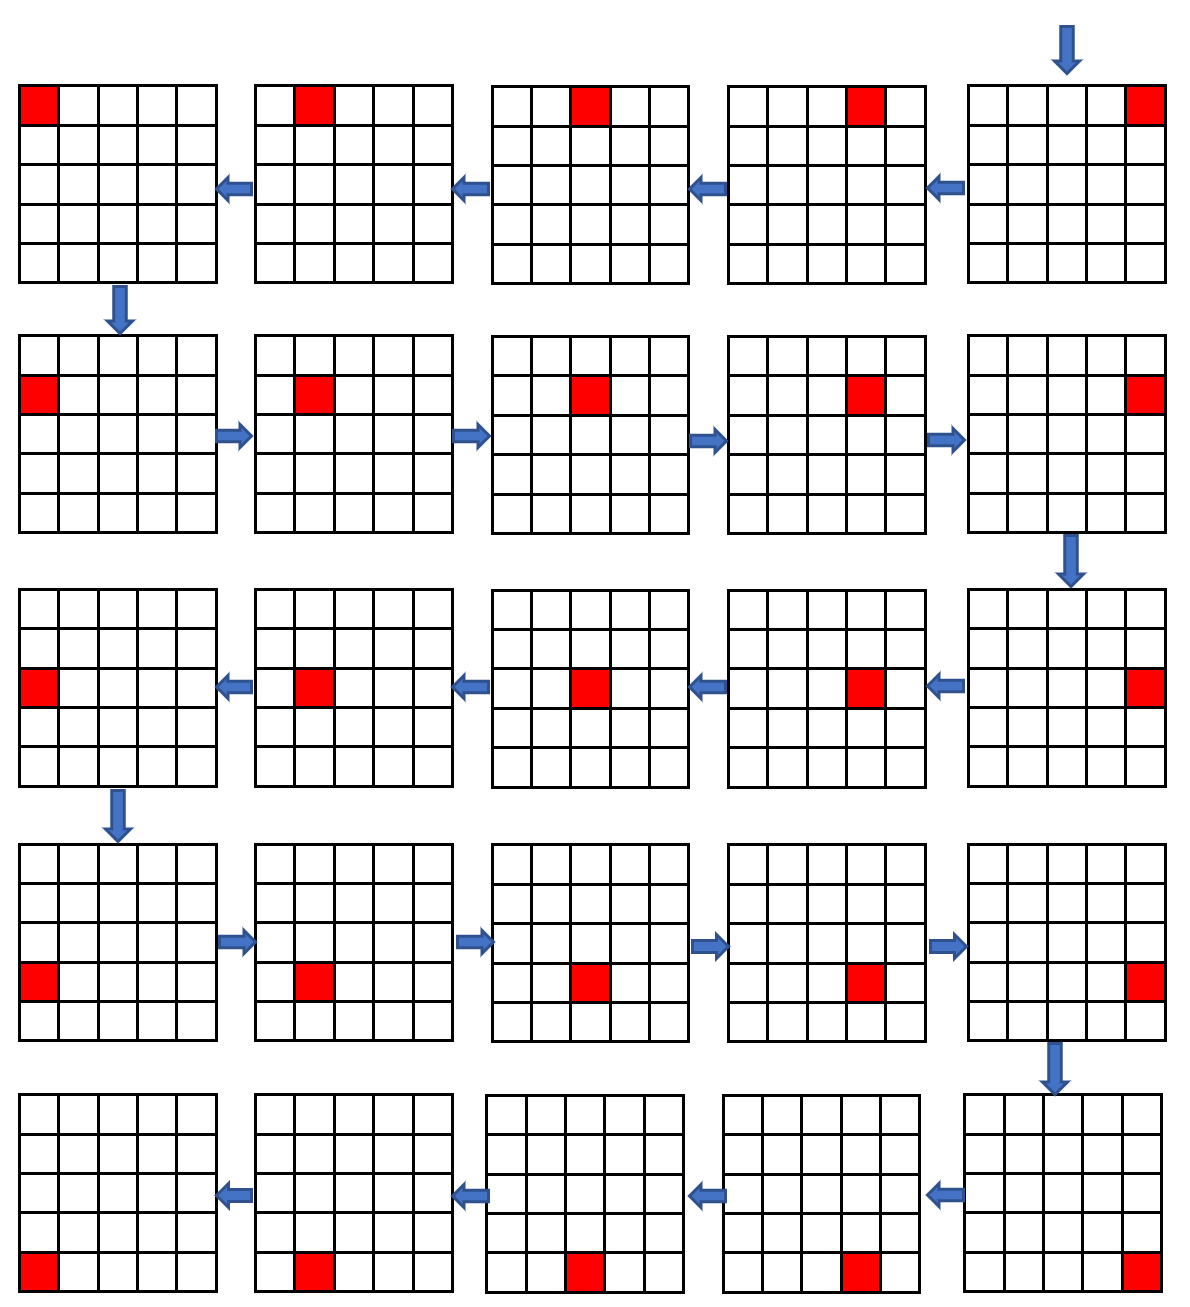
\includegraphics[width=0.6 \linewidth]{figuren/looplicht}
\centering
\caption{De volgorde van het looplicht.}
\label{fig:loopl}
\end{figure}

Begin rechtsboven (bit 0 van de ${0^{e}}$ rij in de matrix) en zet vervolgens steeds de LED links aan. Doe dit tot laatste LED van de rij.
Ga 1 rij naar beneden en zet vervolgens de LED rechts van de rij aan. Doe dit tot en met het $1^{e}$ bit.
Ga 1 rij naar beneden en zet vervolgens de LED links van de rij aan. Doe dit tot en met de laatste LED en ga vervolgens een rij naar beneden.
Doe dit tot en met de laatste rij en begin vervolgens weer op de eerste rij, zoals in het volgende filmpje \href{https://www.youtube.com/shorts/8ZyYWEiXsm0} {
	looplicht}
	te zien is.\\
\textbf{Upload het resultaat op blackboard.}
\end{enumerate}

\paragraph{Challenge opdracht}\label{opdr:accSens}

Op de micro:bit zitten verschillende sensoren. Eén van de sensoren is een \href{https://youtu.be/9WAckt2vrrQ}{accelerometer sensor}.
Het programma in listing \ref{lst:acc} toont de x,y en z waarde van de accelerator sensor.
\begin{enumerate}

	\item Download  listing \ref{lst:acc} van \href{https://github.com/JohnVi-hhs/embsysP/tree/main/voorbeelden/accelerator.ino}{ GitHub} of van brightspace of kopieer listing \ref{lst:acc} in een nieuwe arduino omgeving en voer deze uit.
	\item Pas het programma zodanig aan, zodat de LED in de richting beweegt, waarin micro:kit gehouden wordt.

	\end{enumerate}

\begin{lstlisting}[caption={Looplicht van de bovenste rij.},label={lst:acc}]
#include <LSM303AGR_ACC_Sensor.h>

#define DEV_I2C Wire1   // Wire1 is voor de interne I2C bus 
#define LED ROW1 


// Nodig voor de accelerator 
LSM303AGR_ACC_Sensor Acc(&DEV_I2C);


const int COL1 = 4;   
const int ROW1 = 21;   

void setup() {
	// Led.
	
	pinMode(COL1, OUTPUT);
	digitalWrite(COL1, LOW);
	pinMode(ROW1, OUTPUT);
	
	// Initialisatie van de serieele.
	Serial.begin(9600);
	
	// Initialisate I2C bus (wordt veel gebruikt om sensors).
	DEV_I2C.begin();
	
	// Initialisatie van de accelarator.
	Acc.begin();
	Acc.Enable();
	
	uint8_t a;
	Acc.IO_Read(&a,0x0F,1);
	Serial.print("Ik ben: ");
	Serial.println(a);
}

void loop() {
	// Led blinking.
	digitalWrite(LED, HIGH);
	delay(250);
	digitalWrite(LED, LOW);
	delay(250);
	
	// Lees de accelerometer van de LSM303AGR uit.
	int32_t accelerometer[3];
	Acc.GetAxes(accelerometer);
	
	// Output data.
	Serial.print("| Acc[x/y/z] ");
	Serial.print(accelerometer[0]);
	Serial.print(" ");
	Serial.print(accelerometer[1]);
	Serial.print(" ");
	Serial.print(accelerometer[2]);
	Serial.println(" |");
}
\end{lstlisting}




\bibliographystyle{unsrt}
\bibliography{reference}

\newcommand{\startappendix}{%
%	\cleardoublepage
	\appendix
%	\phantomsection\addcontentsline{toc}{part}{APPENDIX}
%	\part*{APPENDIX}
%	\let\@makechapterhead\@makeschapterhead
}

%\appendix
%\newpage
%\renewcommand{\thechapter}{A}
%\addcontentsline{toc}{section}{Appendices}
%\renewcommand{\thesection}{\Alph{section}}
%\renewcommand{\thesubsection}{\Alph{subsection}}
%\renewcommand{\thesubsection}{\arabic{subsection}
%\renewcommand{\thesection}{\Alph{section}.\arabic{section}}
%\renewcommand{\thesection}{\arabic{section}.\arabic{section}}
%\setcounter{section}{0}

\begin{appendices}
%\section*{Appendices}
%\startappendix

%\printnomenclature
\chapter{De practicum omgeving}
\label{chap:omgeving}
%De practicumopdrachten worden gedaan 
De practicumomgeving van dit instructie college bestaat uit een laptop waarbij de BBC:microbit via een USB micro snoertje is aangesloten, zoals te zien is in figuur \ref{fig:aansluiting}.
	\begin{figure}[h!]
	\captionsetup{justification=centering}
	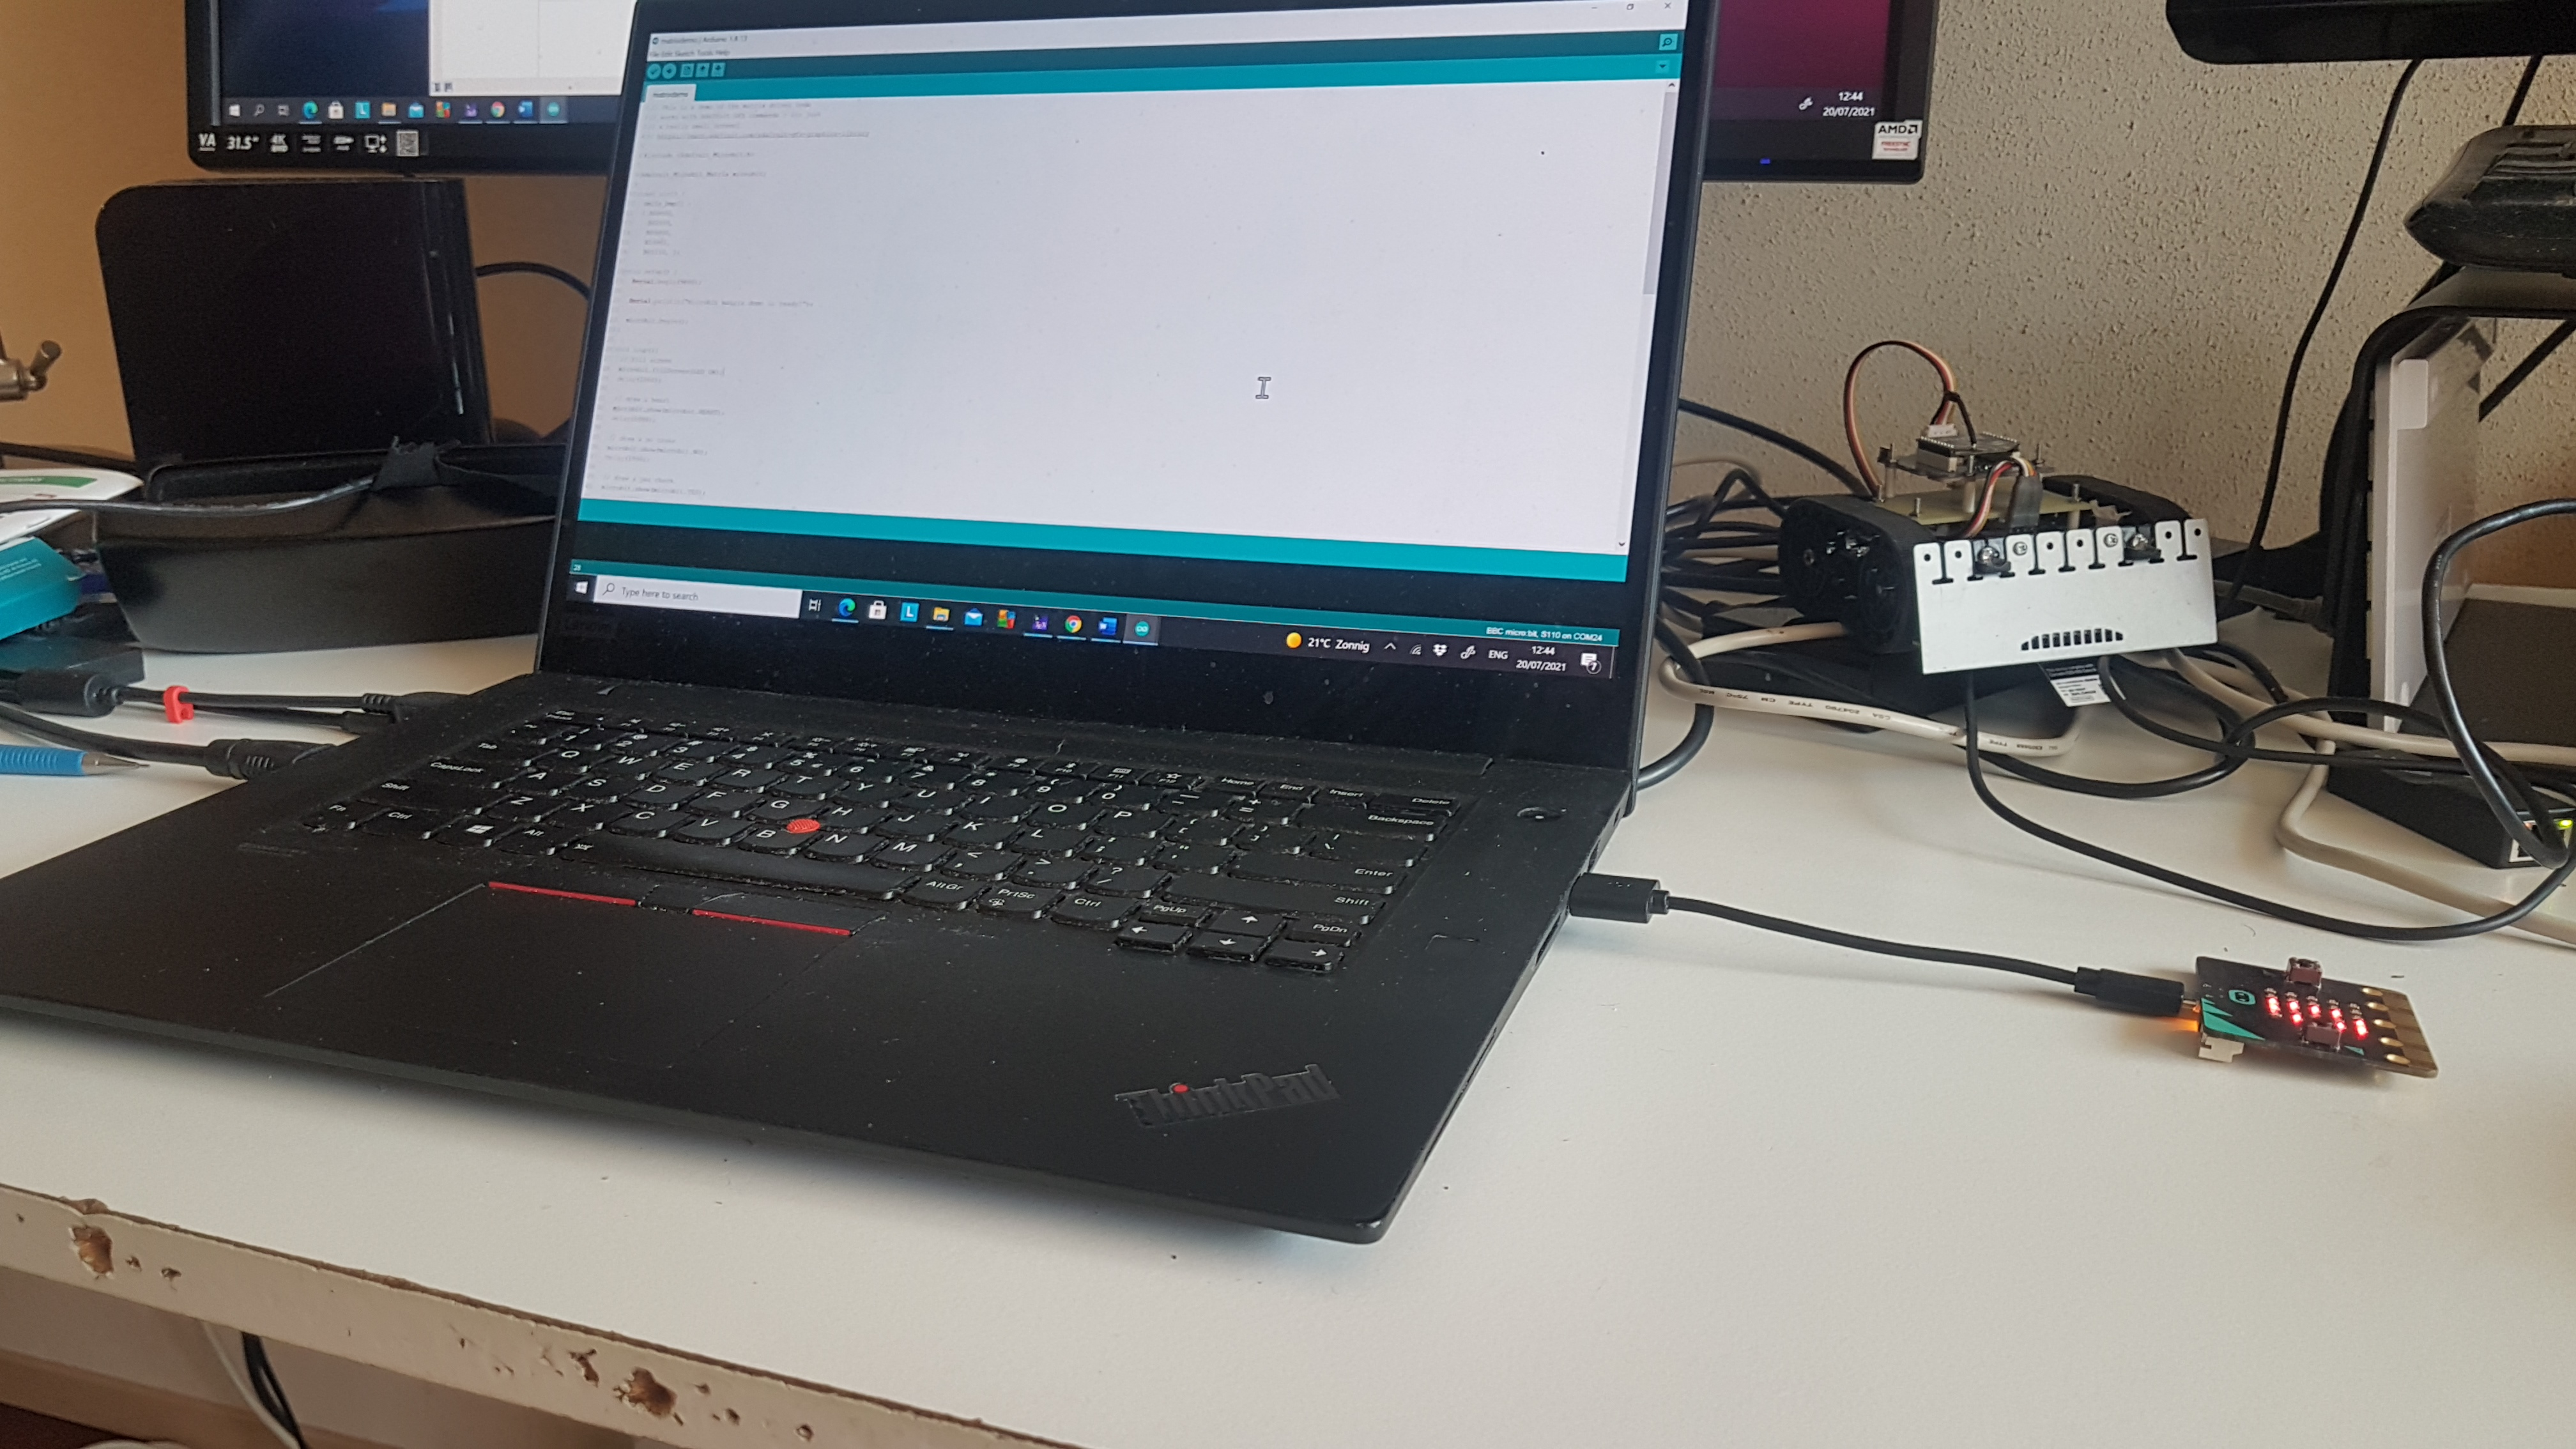
\includegraphics[width=0.40 \linewidth]{figuren/aansluitingBBC}
	\centering
	\caption{aansluiting van de BBC microbit.}
	\label{fig:aansluiting}
\end{figure}
Er zijn verschillende ontwikkelomgeving voor de BBC microbit, maar tijdens dit instructie college(practicum), zal voornamelijk via de \href{https://https://www.arduino.cc/en/software}{Arduino omgeving} omgeving gewerkt worden.


\section{Start met de BBC microbit}

De BBC Microbit is ontwikkeld om programmeeronderwijs te kunnen geven aan leerlingen van groep 7 (10/11-jarigen). Sinds 2016 wordt dit bordje aan elke groep 7 leerling verstrekt, elk jaar ongeveer 1 miljoen stuks. De hardware, het bordje is ‘open source’, de software die we er bij gebruiken ook.

De hardware is robuust, goedkoop, héél eenvoudig te programmeren, je kunt er veel mee en er is prima ondersteuning. Er zijn verschillende ontwikkel omgevingen gebruiken om programma’s te schrijven voor de Microbit. 

Je gaat de Microbit gebruiken in ‘The Challenge’. De Microbit is een Embedded System. Een Embedded System bestaat uit een microcontroller met sensoren en actuatoren. Met sensoren meet je iets (licht, temperatuur, beweging), met actuatoren stuur je iets aan (b.v een ledje, een speakertje, een motor, etc.). Met de Microbit kun je IoT (Internet of Things) devices simuleren, dit zijn ook Embedded Systems. Met een IoT device wordt meestal een apparaat bedoeld die een radiomodule bevat die data kan verzenden of ontvangen. Je kunt deze radiomodule zien als een black box. Er zijn veel verschillende typen voor veel verschillende toepassingen. Ze verschillen in bereik, datadoorvoer, reactiesnelheid en energieverbruik. 
Voor ‘The Challenge’ maakt het niet uit, je kunt met de Microbit prima een IoT device simuleren.

Let op: Het installeren van software moet je zelf uitzoeken, dit kost veel tijd. Verwacht daarom niet dat je docent je hiermee kan helpen!

Indien het niet lukt, kan altijd om hulp gevraagd worden, maar doe dat met specifieke vragen en vertelt erbij wat jezelf al uitgeprobeerd heb.


\subsection{Eerste kennismaking met de Microbit}

Sluit de microbit met behulp van een USB micro snoertje aan op je laptop, zoals te zien is in figuur \ref{fig:aansluiting}.
Windows herkent de microbit en kent daar een \textbf{drive letter} voor, zoals ook gebeurt bij een USB stick. Dit is te zien in figuur \ref{fig:driveL}.


\begin{figure}[h!]
	\captionsetup{justification=centering}
	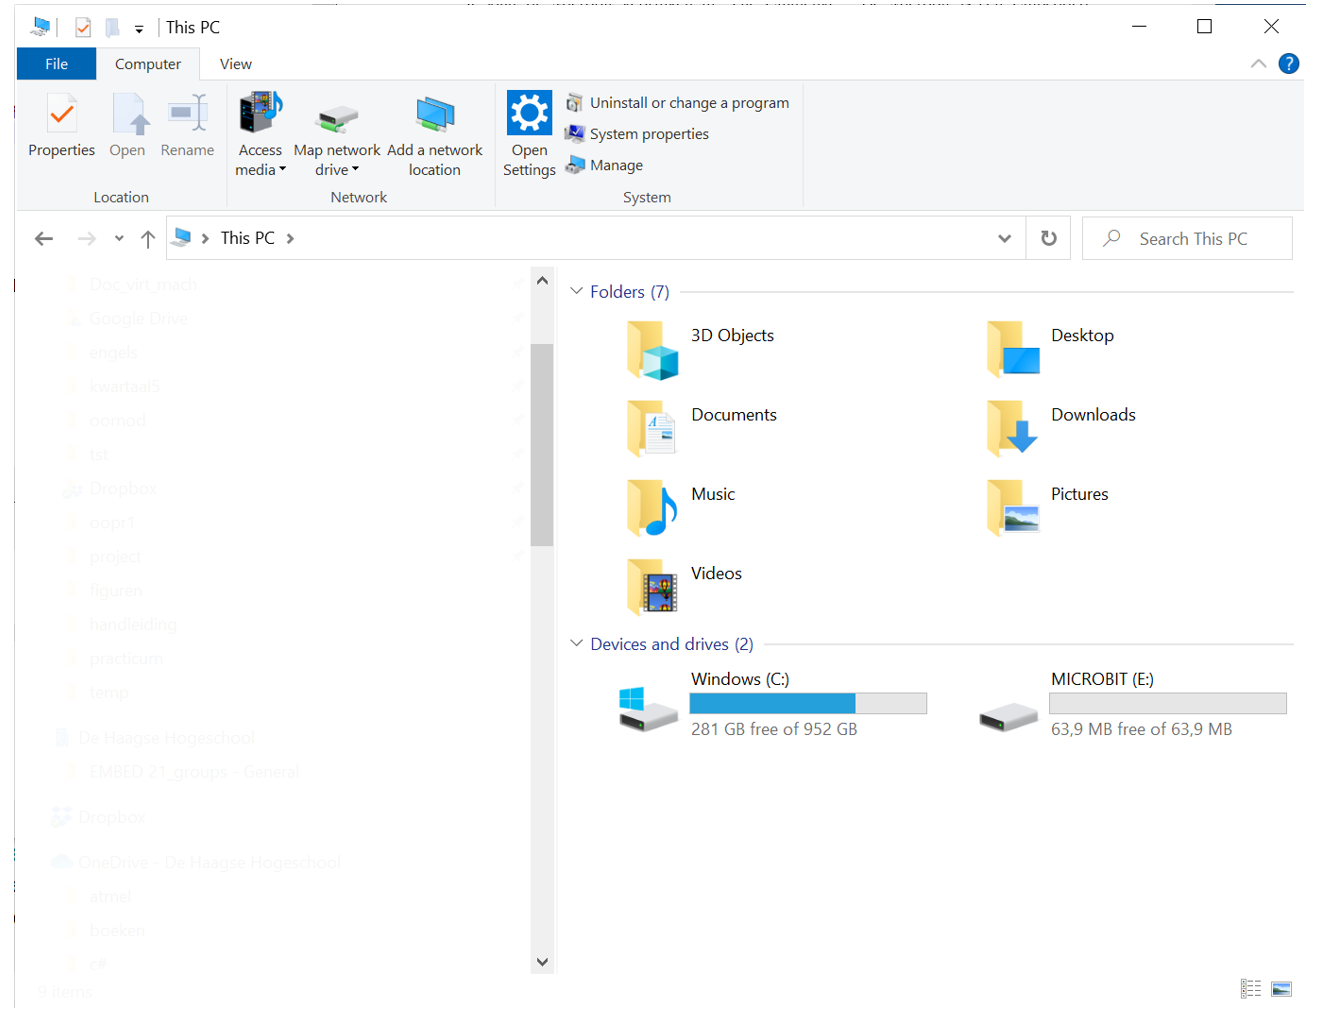
\includegraphics[width=0.50 \linewidth]{figuren/driverLetter}
	\centering
	\caption{Herkenning microbit in windows.}
	\label{fig:driveL}
\end{figure}

Na het aansluiten zal bij een nieuwe BBC microbit de ingebouwde demo gaan lopen. Werkt de ingebouwde demo niet, dan kan je naar de \href{https://support.microbit.org/support/solutions/articles/19000021613-reset-the-micro-bit-to-factory-defaults}{Reset de micro:bit to factory pagina} gaan en download het  \href{https://support.microbit.org/helpdesk/attachments/19067609189} {OutOfBoxExperience.hex} programma en zet dit op de MICROBIT drive. Hierdoor zal het programma geüpload worden op de microbit.

Voor verdere kennismaking met de microbit is de de pagina \href{https://microbit.org/get-started/first-steps/set-up/}{https://microbit.org/get-started/first-steps/set-up/}
een goed startpunt.


\subsection{De Microbit in “The Challenge”}

De doelstelling van The Challenge is dat hier producten van alle differentiaties in samenkomen. Voor het NSE/Embedded deel houden we het eenvoudig.


Je zou tijdens de Challenge eventueel ook de microbit met \href{https://docs.arduino.cc/micropython/?_gl=1*bbja8p*_gcl_au*MTA0MzMyMzUwNC4xNzI4NDYwNDQ0*FPAU*MTA0MzMyMzUwNC4xNzI4NDYwNDQ0*_ga*MTM2NDc5NzM2OC4xNzI4NDYwNDQy*_ga_NEXN8H46L5*MTcyODQ2MDQ0MS4xLjEuMTcyODQ2MDQ5MS4wLjAuMTk3NzAxMDU1NQ..*_fplc*dmdpUTJCaSUyQjFINjd2SExxV092Zml5Ym92VlZQMGdtNWFSeG0lMkJLWEpQSnFDMkE4cG52M1klMkJGcGdNYzRKNGhBTkMzRXcyOXc0Ykhvcndmc0UyMVdwM1U2Rzc0bkFURWoxRHBWN3RlbjNvMlRNOVJ0eW1nSmp3OXFucURhWW9BJTNEJTNE}{micropython} kunnen programmeren.
Verder is er nog een mogelijkheid om de “blokken” taal te gebruiken. Hier kun je ook alles mee.
Voor een intro in de “blokken” taal, start hier en begin met ‘Mode’, ‘Step Counter’, kies voor ‘Instructies weergeven’: \href{https://makecode.microbit.org/}{https://makecode.microbit.org/}

Het ligt voor de hand dat NSE studenten in de Arduino omgeving programmeren, waar de programmeertalen C/C++ de voertaal is.\\

\section{Kennismaken met de Arduino omgeving}

De Arduino omgeving oftewel Arduino IDE (Integrated Development Environment) kan je gebruiken om de Microbit te programmeren. 
%Mocht je de software nog niet geïnstalleerd hebben, volg dan de instructies in “Installatiehandleiding Arduino software voor BBC Microbit”.

We gebruiken de Arduino IDE omdat deze op beginnersniveau zeer veel gebruikt wordt en er veel voorbeeldcode te vinden is.
 
Eigenlijk maakt de Arduino IDE gebruik van de taal C++, dit is een Object Oriented uitbreiding van de taal C. Het C++ / Object Oriented deel van de programmeertaal zie je soms terug in instructies zoals Serial.begin(9600); De punt tussen Serial en begin is hier een indicatie van.

Java en C++ zijn object georiënteerde talen. Daarover leer je meer als je kiest voor de differentiaties “Software Engineering” of “Networks \& System Engineering”. Voor dit practicum houden we het eenvoudig. We gebruiken de taal zoveel mogelijk als klassieke “imperatieve” programmeertaal waarbij gewerkt wordt met een reeks opeenvolgende instructies.



\subsection{Het installeren van de Arduino omgeving}

VOER ONDERSTAANDE INSTALLATIE THUIS UIT – DIT DUURT 1,5 UUR!!!

\begin{enumerate}
	\item Download de Arduino software van \href{https://www.arduino.cc/en/software}{https://www.arduino.cc/en/software}, zoals je kan zien zijn er ook versies voor Linux en de Mac.
	\item  Bevestig alle vragen, klik maar door.
	\item Bij het het opstarten van arduino zal gevraagd worden om de libary's te updaten. Update de libary's.
\end{enumerate}
Na het opstarten verschijnt het scherm zoals in figuur \ref{fig:arduino_s1} wordt weergegeven.

\begin{figure}[h!]
	\captionsetup{justification=centering}
	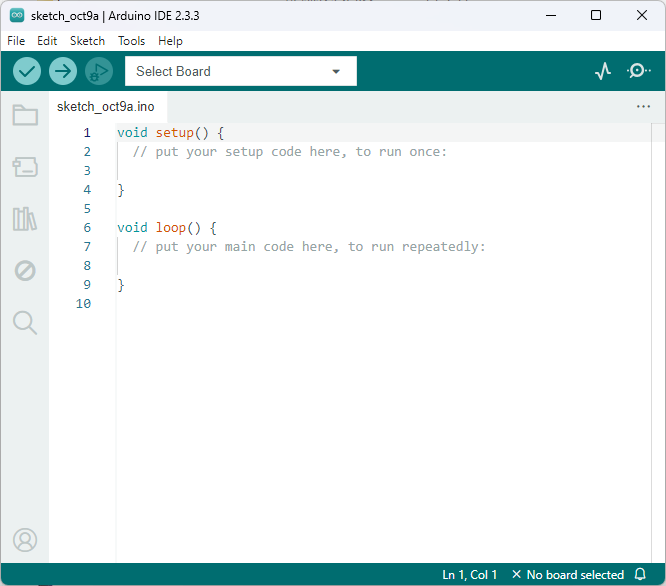
\includegraphics[width=0.50 \linewidth]{figuren/arduino_s1}
	\centering
	\caption{De Arduino omgeving met een leeg scherm.}
	\label{fig:arduino_s1}
\end{figure}
Waarin de functie \lstinline |void setup() {}| één keer wordt uitgevoerd en de functie \lstinline |void loop() {}| continu wordt uitgevoerd.


Als eerste kunnen een aantal instellingen aangepast worden. Ga naar File $\rightarrow$ Preferences, en pas de instellingen aan zoals te zien is in figuur \ref{fig:arduinoPref}.
\begin{figure}[H]
	\captionsetup{justification=centering}
	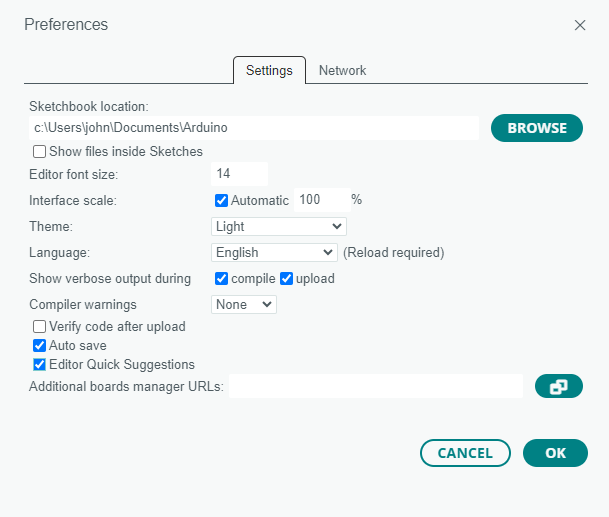
\includegraphics[width=0.50 \linewidth]{figuren/arduinoPref}
	\centering
	\caption{preferences scherm.}
	\label{fig:arduinoPref}
\end{figure}

\begin{itemize}
	\item Indien de Arduino omgeving Engelstalig is, kan deze gewijzigd worden naar het Nederlands. Het is handig om tijdens de installatie de Engelstalige omgeving te gebruiken.
\end{itemize}
\subsection{De arduino omgeving geschikt maken voor de microbit.}

De firma \href{https://www.adafruit.com/about}{Adafruit } ontwikkelt diverse componenten voor met name embedded systemen
die door ieder gebruiker kan worden toegepast en/of geprogrammeerd. Om dit waar te kunnen maken worden veel tutorials ontwikkeld. Zo is er ook een uitgebreide website, om de \href{https://learn.adafruit.com/use-micro-bit-with-arduino}{microbit met de Arduino IDE} te programmeren.

Doordat op de microbit een NRF52 microcontroller zit, zal de betreffende package bij de arduino omgeving bekent moeten worden gemaakt, waarna de betreffende board met deze microcontroller geselecteerd kunnen worden.
\begin{enumerate}
	\item  Ga naar File $\rightarrow$ Preferences, en zet bij Additional boards manager URLs: de URL  %\texttt{https://sandeepmistry.github.io/arduino-nRF5/package\_nRF5\_boards\_index.json
    {\scriptsize \texttt{https://sandeepmistry.github.io/arduino-nRF5/package\textunderscore nRF5\textunderscore boards\textunderscore index.json}}  zoals in figuur \ref{fig:arduinoPref2} te zien is.\\ 

	\begin{figure}[H]
		\captionsetup{justification=centering}
		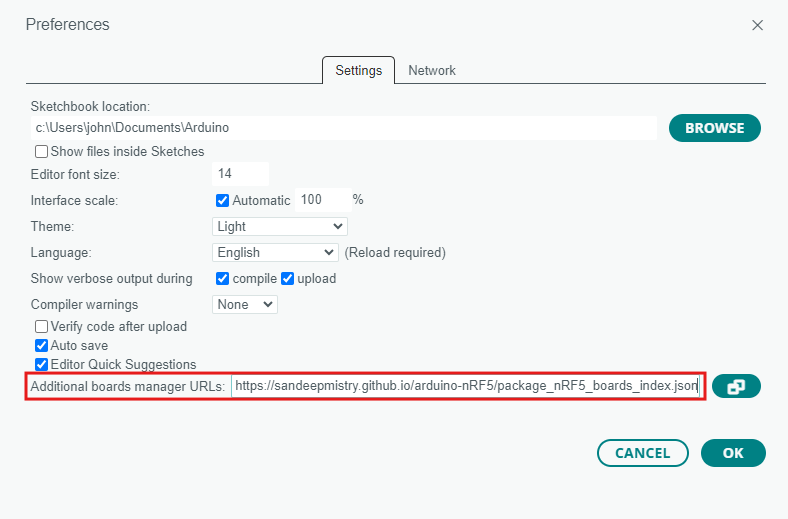
\includegraphics[width=0.60 \linewidth]{figuren/arduinoPref2}
		\centering
		\caption{preferences scherm.}
		\label{fig:arduinoPref2}
	\end{figure}
	
   \item Het selecteren van diverse borden met een nRF5 microcontroller  wordt als volgt gedaan: Ga naar Tools $\rightarrow$ Boards $\rightarrow$ Boards manager.. zoals figuur \ref{fig:ardTool1} aangeeft.
\begin{figure}[h!]
	\centering
	\begin{center} 	
		\begin{subfigure}[b]{0.48\textwidth}
			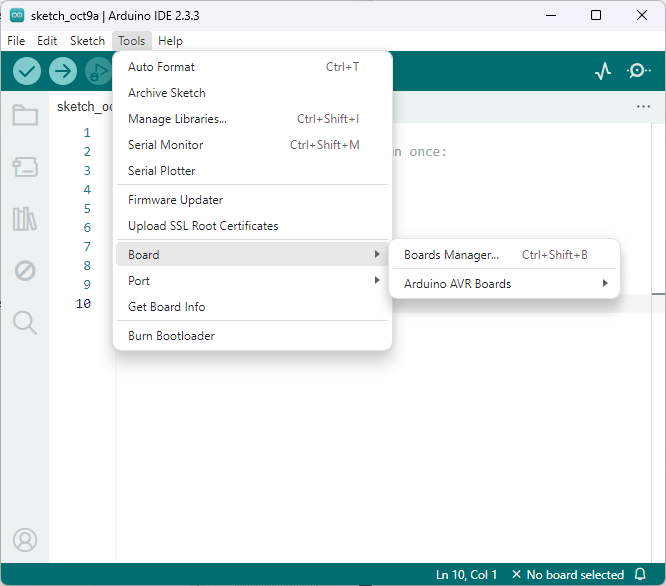
\includegraphics[width=0.8\textwidth]{figuren/arduinoTools}
			\caption{selecteren van de board manager }
			\label{fig:ardTool1}
			
		\end{subfigure}
		\begin{subfigure}[b]{0.48\textwidth}
			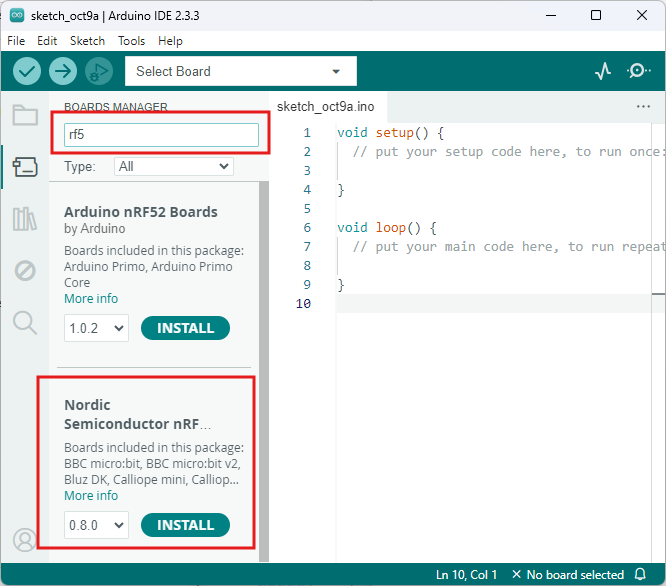
\includegraphics[width=0.8\textwidth]{figuren/arduinoTools2}
			\caption{Installeren van de NRF5 borden }
			\label{fig:ardTool2}
		\end{subfigure}
		\captionsetup{justification=centering}
		\caption{Arduino laten werken met de microbit. }
		\label{fig:ardTool}
	\end{center}
	
\end{figure}
Zoek op \textit{nrf} en installeer vervolgens de \textbf{Nordic Semicinductor nRF}, zoals in figuur \ref{fig:ardTool2} wordt weergeven.

\item Het selecteren van de microbit als het bordje waarop geprogrammeerd wordt, wordt als volgt gedaan: Ga naar Tools $\rightarrow$ Boards $\rightarrow$ Nordic Semiconductor NRF5 Boards en selecteer BBC micro:bit V2 zoals figuur \ref{fig:ardTool3} wordt weergegeven.
\begin{figure}[H]
	\captionsetup{justification=centering}
	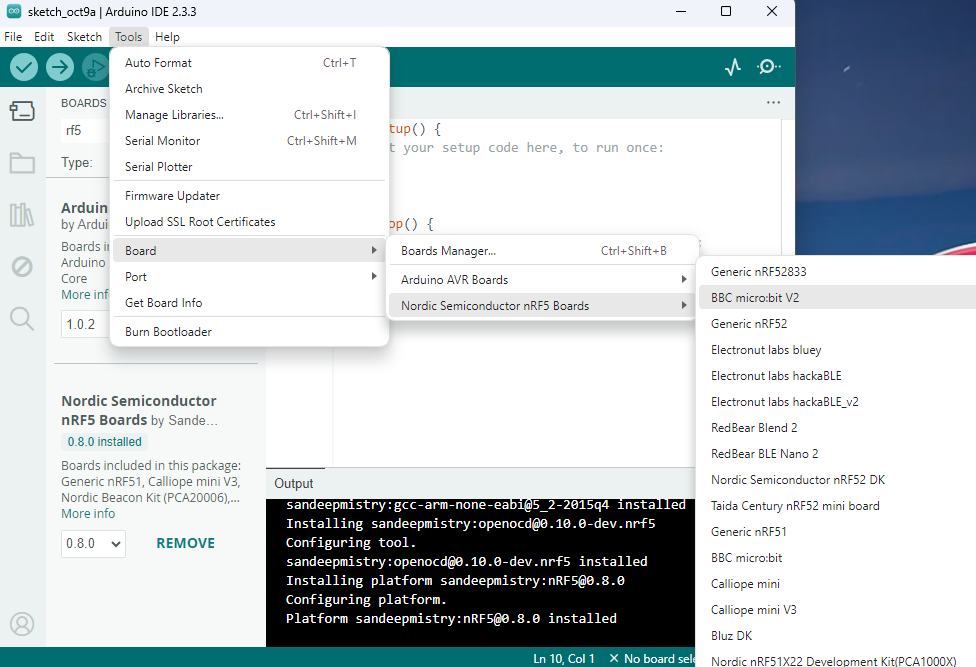
\includegraphics[width=0.60 \linewidth]{figuren/arduinoTools3}
	\centering
	\caption{Selecteren van de micro:bit als bord waarop gewerkt wordt.}
	\label{fig:ardTool3}
\end{figure}

\item Controleer of de arduino aangesloten is op de USB port en selecteer de juiste COM port. Ga naar Tools $\rightarrow$ Port $\rightarrow$ (BBC micro:bit,....))

In figuur \ref{fig:ardTool4} is te zien dat de microbit op COM7 zit, dit kan bij iedereen weer anders zijn.
\begin{figure}[H]
	\captionsetup{justification=centering}
	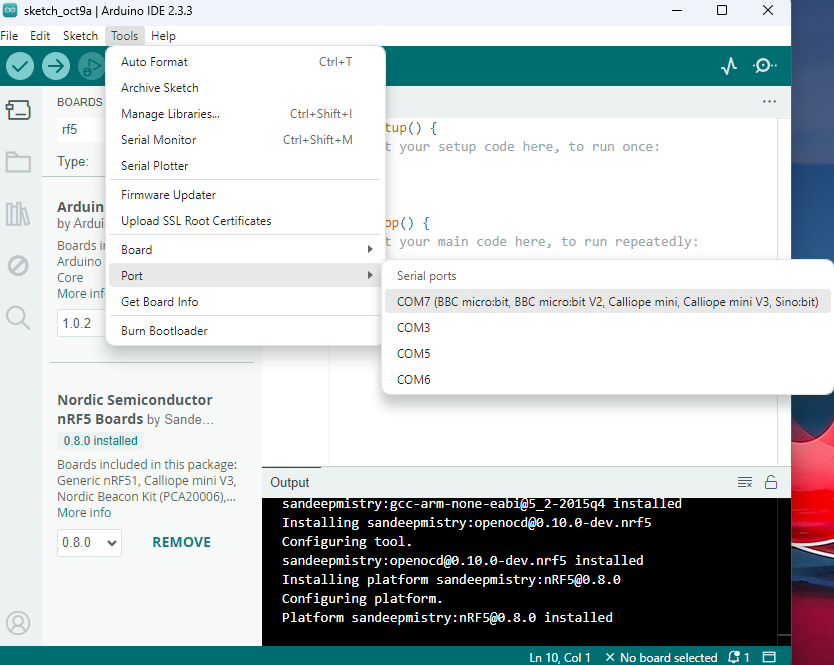
\includegraphics[width=0.60 \linewidth]{figuren/arduinoTools4}
	\centering
	\caption{Selecteren van de micro:bit als bord waarop gewerkt wordt.}
	\label{fig:ardTool4}
\end{figure}

\item Het uploaden van een programma gebeurt door op de knop \img{figuren/ardIcUpl} te klikken. Windows komt met de melding zoals hieronder wordt weergegeven. 
   	\begin{figure}[h!]
   	\captionsetup{justification=centering}
   	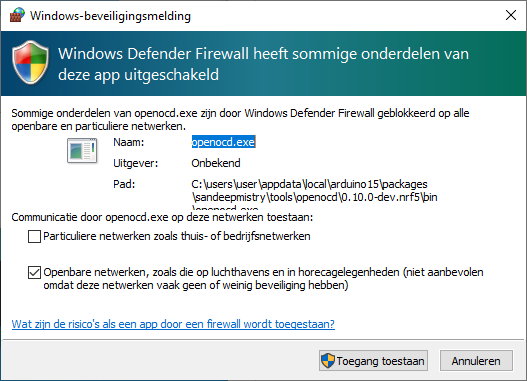
\includegraphics[width=0.45 \linewidth]{figuren/windowsDefSec}
   	\centering
   	\caption{Melding van windows defender.}
   	\label{fig:windowsDef}
   \end{figure}
Hiermee vraagt Windows toestemming om de USB port te mogen gebruiken.
\item Haal de voorbeeldcode van blackboard of \href{https://github.com/JohnVi-hhs/embsysP/tree/main/voorbeelden/blink.ino}{download} de laatste versie en plaats deze in je eigen werkdirectory.
\item \label{en:blink} Open het voorbeeldprogramma blink.ino (dubbel klik), dat wordt weergegeven in Listing \ref{lst:blink}, compileer en upload naar de micro:bit (klik op de knop \img{figuren/ardIcUpl}). \\
Als het goed is gaat het linkerboven LEDje van de matrix knipperen. Voor verder uitleg zie hoofdsuk \ref{sec:blink}


\end{enumerate}

\subsection{Het installeren van de Adafruit library.}

Zodra je complexere zaken wilt aanpakken, heb je een hulplibrary nodig om dingen zoals de interne temperatuursensor, LED-matrix of Bluetooth-verbinding te beheren.
Om het je makkelijker te maken, heeft Adafruit een wrapper-library geschreven die dit allemaal voor je regelt.

\begin{enumerate}
	\item Ga naar Sketch$\rightarrow$ include library $\rightarrow$ Manage Labraries zoals figuur \ref{fig:ardLib} aangeeft
	
	   	\begin{figure}[h!]
		\captionsetup{justification=centering}
		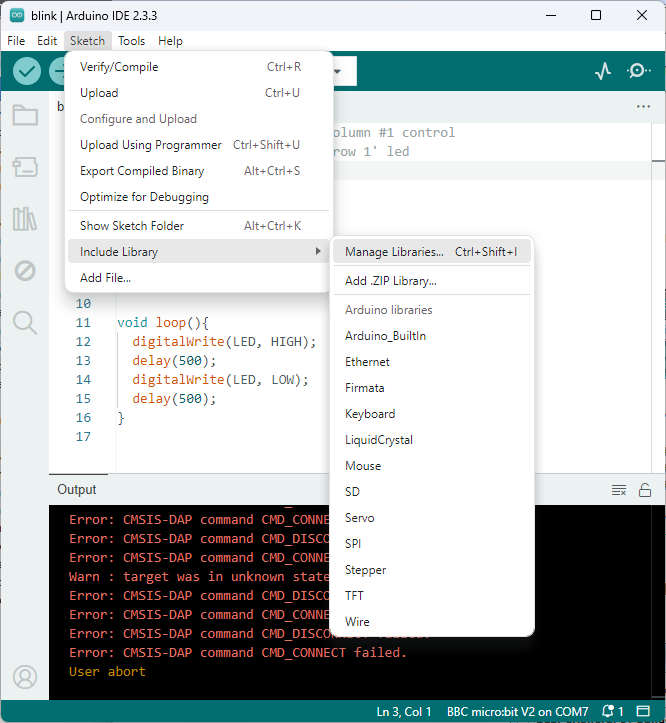
\includegraphics[width=0.45 \linewidth]{figuren/arduino_lib}
		\centering
		\caption{Installeren van van Library.}
		\label{fig:ardLib}
	\end{figure}
	\item Zoek naar de \textbf{Blep} library en installeer deze zoals te zien is in figuur \ref{fig:ardlibBl} de \textbf{Adafruit GFX library}  met de  dependency zoals te zien is in figuur \ref{fig:ardlibAdaf} en de \textbf{Adafruit Microbit} zoals te zien is in figuur \ref{fig:ardlibMicro}.
	
\begin{figure}[h!]
	\centering
		\begin{center} 	
			\begin{subfigure}[b]{0.31\textwidth}
				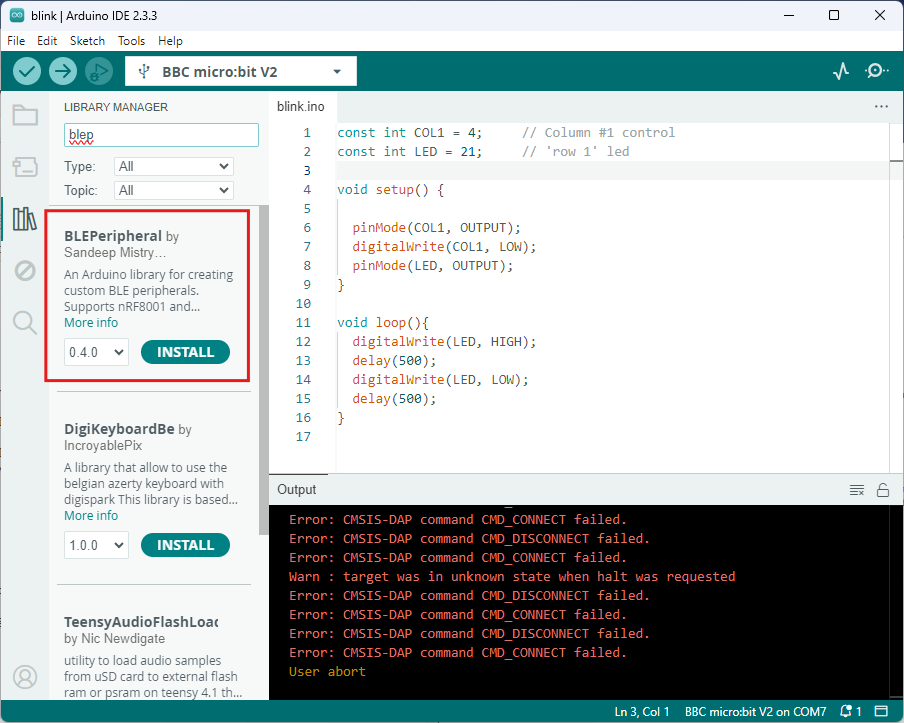
\includegraphics[width=0.98\textwidth]{figuren/arduinoManLibBlep}
				\caption{Installeren van BLEPerpheral }.
				\label{fig:ardlibBl}
				
			\end{subfigure}
			\begin{subfigure}[b]{0.33\textwidth}
				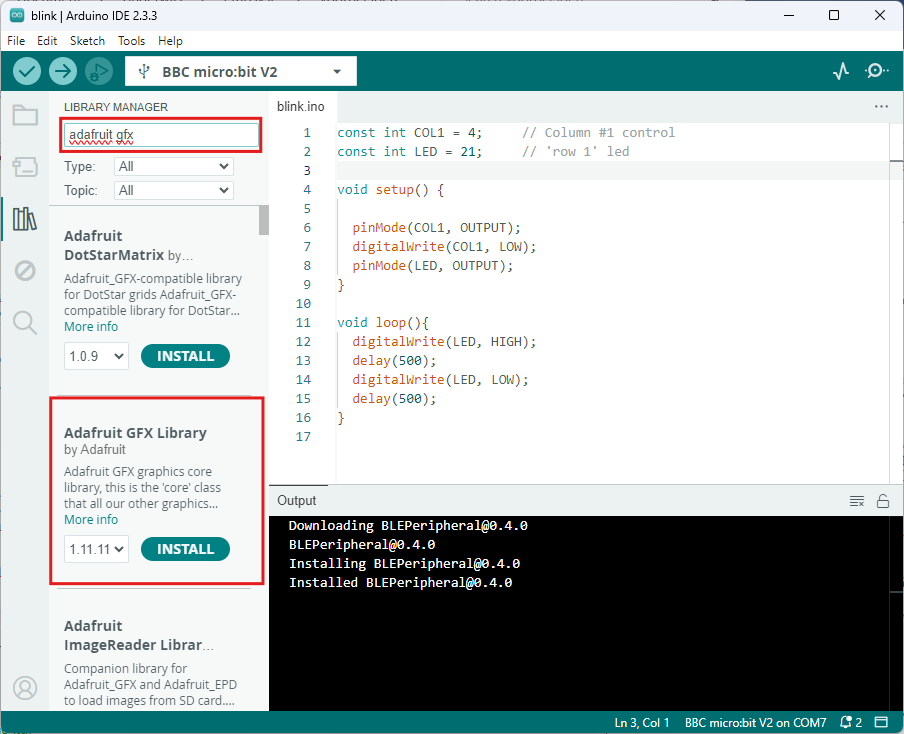
\includegraphics[width=0.98\textwidth]{figuren/arduinoLibAdafruit}
				\caption{Installeren Adafruit microbit }
				\label{fig:ardlibAdaf}
			\end{subfigure}
			\begin{subfigure}[b]{0.33\textwidth}
	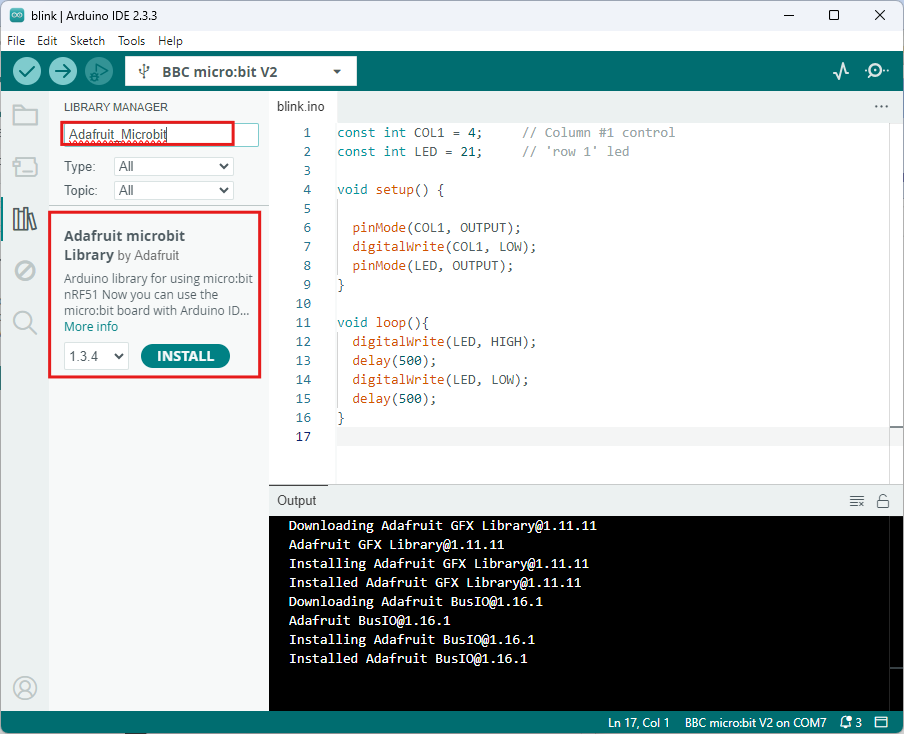
\includegraphics[width=0.98\textwidth]{figuren/arduinoLibAdamico}
	\caption{Installeren Adafruit library }
	\label{fig:ardlibMicro}
\end{subfigure}			
			\captionsetup{justification=centering}
			\caption{Het installeren van Arduino libraries. }
			\label{fig:ardInstal}
		\end{center}
		
	\end{figure}
	
	
\end{enumerate}



\chapter{Problemen tijdens het practicum.}\label{chap:apB}


\section{Adafruit\_Microbit.h: No such file or directory.}~\\
%Adafruit_Microbit.h: No such file or directory
%Adafruit\_Microbit.h: No such file or directory.\\
Contoleer of de Adafruit microbit geïnstalleerd is.
\begin{enumerate}
	\item Ga naar de library manager zoals aangegeven in figuur \ref{fig:ardLibMan}
	\item Controleer of library geinstalleerd is, zolas aangegeven in figuur \ref{fig:ardLibCon}
\end{enumerate}

\begin{figure}[h!]
	 		\centering
	  \begin{center} 	
		\begin{subfigure}[b]{0.45\textwidth}
     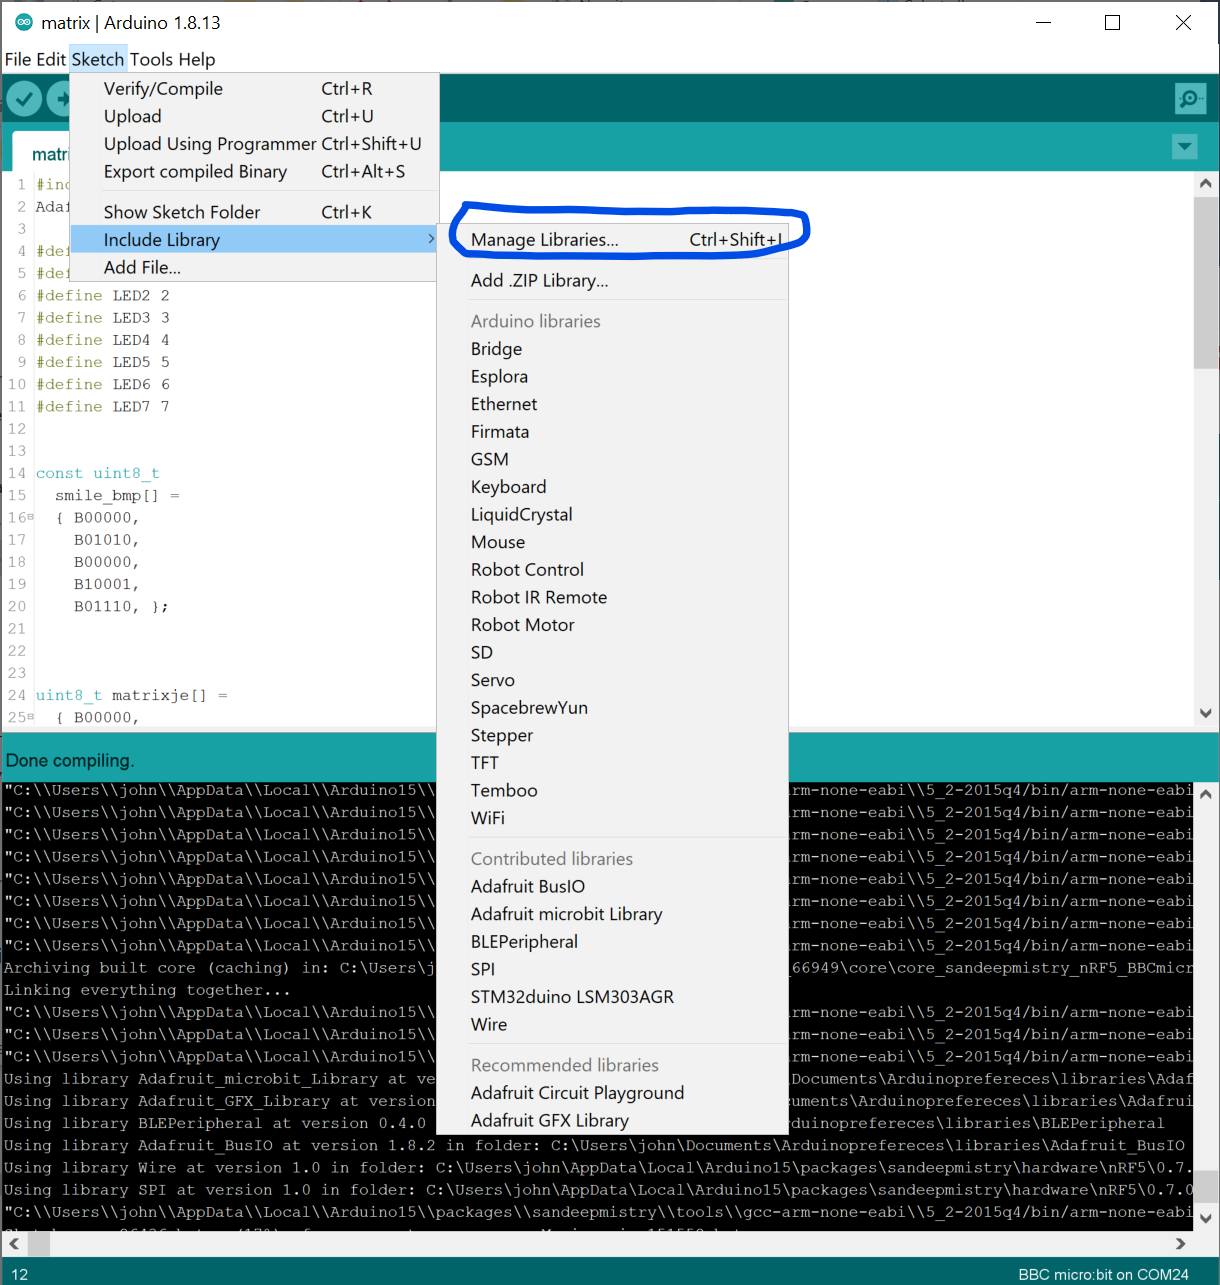
\includegraphics[width=0.7\textwidth]{figuren/arduinoManLib}
    \caption{selecteren van de library manager }
     \label{fig:ardLibMan}
   \end{subfigure}
\begin{subfigure}[b]{0.54\textwidth}
	     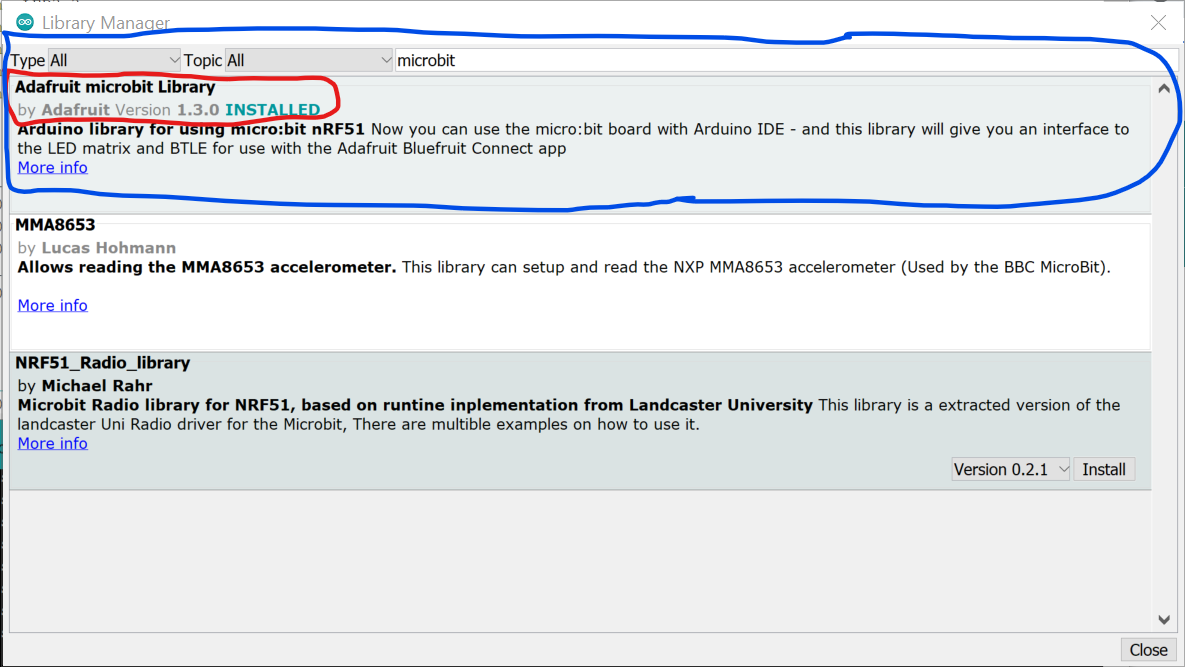
\includegraphics[width=0.98\textwidth]{figuren/arduinoManLibIns}
	\caption{Constrole Library is geïnstalleerd }
	\label{fig:ardLibCon}
\end{subfigure}
\captionsetup{justification=centering}
\caption{Controleren of library is geïnstalleerd. }
\label{fig:ardinopr1}
\end{center}

\end{figure}

\section{SerialPortException: Port name - COM..}~\\
java.io.IOException: jssc.SerialPortException: Port name - COM24; Method name - setEventsMask(); Exception type - Can't set mask.

De seriële poort is in gebruik door waarschijnlijk de monitor.

Sluit de monitor af.
 
 
\section{Tijdens het uploaden}
 Error: unable to find CMSIS-DAP device
 Error: No Valid JTAG Interface Configured.
 Error: No Valid JTAG Interface Configured.
 
 Haal de USB stekker uit de laptop en doe deze opnieuw erin.
 
 \section{Tijdens compileren  'kan stdint.h niet vinden'}
 Mogelijk is er iets fout gegaan bij het installeren van de \textbf{Add NRF5x Board Support}. Waardoor de library niet geinstalleed is.
 
 Bij het installeren van de 'Add NRF5x Board Support' moet er een lange tijd gewacht worden. Mogelijk is deze onderbroken. Bij het opnieuw installeren lijk alles goed te gaan, dit is echter niet zo.
 
 Mogelijke oplossing:\\
 remove het board en installeer deze opnieuw (wacht nu wel totdat deze geïnstalleerd is).
 
 
%\chapter{Vereisten aan code voor ‘The Challenge’}

Hieronder is aangegeven waaraan jouw code moet voldoen. Dit is deel van de beoordeling!

\begin{itemize}
	\item Bronvermelding
	
Je kunt de opdrachten maken door de Arduino voorbeelden te bestuderen en slim samen te voegen. Je mag (moet!) dus code kopiëren. Vermeld in commentaar boven of achter je code waar je de code vandaan hebt. Je kunt bijvoorbeeld de naam van het voorbeeld opgeven of de URL van de webpagina waar je het vandaan hebt. Geen bronvermelding is (ook bij softwareontwikkeling!) plagiaat.

\textit{Zorg dat jouw programma de structuur heeft zoals de voorbeeldcode van Arduino. }

\item Gebruik van commentaar

Commentaar staat tussen /* en */ en kan zo over meerdere regels staan of zelfs in een regel tussen programmacode, zoals in het voorbeeld hieronder:\\
pinMode(LED\_BUILTIN /* dit is eigenlijk pin 13 */, OUTPUT);
De andere manier om commentaar aan te geven is met // 
Alles wat achter deze 2 slashes staat wordt als commentaar gezien en wordt door de compiler volledig genegeerd. Zo kan je ook (tijdelijk) regels in je programma uitzetten om iets uit te proberen.

\item Layout van je programma.

Een nette layout zorgt voor een goede leesbaarheid. In de Arduino omgeving is daar een eenvoudig hulpmiddel voor:  ga naar “Tools”, “Auto Format” of druk Ctrl+T.
\item Kwaliteit van code

Zorg dat dezelfde code niet op meerdere plaatsen gebruikt wordt. Dat maakt code slecht leesbaar en zeker op microcontrollers gaat dat ten koste van de schaarse geheugenruimte. Gebruik functies.

\item Naamconventies

Geef functies en variabelen een betekenisvolle naam en schrijf deze namen in camelCase (elk woord begint met een hoofdletter, behalve de eerste letter). Voorbeelden: 
int pinCount;\\
int myFunction();
Constanten schrijf je in hoofdletters, woorden scheiden met underscore “\_”. Voorbeeld: \\
\#define BEEP\_PIN 3 

\item Versiebeheer

Geef bestanden een betekenisvolle naam, liefst met een versienummer, zodat je ze later eenvoudig kunt terugvinden. Voorbeeld: “Thermometer-v0.1”. Doe dit met al je bestanden!

\textbf{Tip:} Sla je programma regelmatig, na elke nieuwe tussenstap op met een nieuw versienummer. 
Zo kan je altijd terug naar een werkende versie als er iets misgaat. 

Beschrijf wijzigingen en versies als commentaar in je programma, dan hoef je niet veel te zoeken!
\end{itemize}
%\chapter{Data vanuit de Microbit naar SQL sturen}

Dit is het meest complexe deel van de software die je nodig hebt voor ‘The Challenge’. 

Hierin komen 3 vakgebieden samen: Embedded, Java en Databases (SQL).

Bedenk: Dit is slechts een voorbeeld dat laat zien hoe je dat voor de verschillende delen aanpakt.

We gaan er mee om zoals met de eerdere Arduino voorbeelden, zie dit als legoblokjes:

\begin{itemize}
	\item Maak je eigen code erbij voor de Microbit. 
\item In het Java deel voegen jullie een GUI toe.
\item In de database bouwen jullie een structuur met minstens 2 tabellen.
\end{itemize}

Het plaatje hieronder geeft weer wat we gaan doen, zie deze stappen: 

Stap 1: De Microbit meet temperatuur en geeft dit per seconde door via de seriële poort naar de PC. 

Stap 2: Op de PC draait een Java programma die de seriële data vertaalt naar iets bruikbaars.

Stap 3: Het Java programma stopt de data in de SQL database.


\begin{figure}[h!]
	\captionsetup{justification=centering}
	\includegraphics[width=0.6 \linewidth]{figuren/microToSQL}
	\centering
	\caption{Micro:bit naar SQl}
	\label{fig:microSQL}
\end{figure}

Om te zien hoe dit werkt, kijk naar het filmpje \href{https://youtu.be/wZ_bIQh9tME}{"Microbit: Embedded + Java + SQL datalogging"}


\section{Software installeren}

Ik ga er vanuit dat je de volgende software geïnstalleerd hebt:

\begin{itemize}
\item IntelliJ IDE voor Java
\item MySQL database
\end{itemize}

Zo niet, dan staat hieronder waar je het kunt vinden. Zoek zelf uit via de instructies van het vak wat daar precies vereist is.

\paragraph{IntelliJ: }

Deze hebben jullie al geïnstalleerd, daarom geen instructies. Mocht je het nog niet hebben, dit is de link:
\href{https://www.jetbrains.com/idea/download/index.html}{https://www.jetbrains.com/idea/download/index.html}


\paragraph{MySQL:}

Als je Windows gebruikt, download en installeer dan de MySQL Installer (web community versie) vanaf:
\href{https://dev.mysql.com/downloads/installer/}{https://dev.mysql.com/downloads/installer/}


In de installer, selecteer de nieuwste versie van:

\begin{itemize}

\item -MySQL Server
\item -MySQL Workbench

\end{itemize}

(Op 7-12-2019 is dat versie 8.0.18)

\section{Voorbeeld downloaden}


Ga in Blackboard naar de map “Benodigheden voor The Challenge”, “Tips, voorbeeldcode etc.” 

Lees de tekst in de sectie “Informatie, hulpmiddelen en voorbeeldcode”.


Download de voorbeeldcode 
\href{https://blackboard.hhs.nl/bbcswebdav/pid-2889780-dt-content-rid-24452591_2/xid-24452591_2
}{USBserialReceiveToSQL.zip}

Dit bevat het complete project voor het uitlezen van data vanuit de seriële poort en dit in SQL stoppen.

Pak het zip bestand USBserialReceiveToSQL.zip uit naar waar je wilt (map met andere java projecten?)
Je hebt daar nu een map USBserialReceiveToSQL

Start IntelliJ, blader naar bovenstaande map (selecteer de map USBserialReceiveToSQL) en klik OK.

Kies “New window” om het project in een nieuwe instantie van IntelliJ te starten.

\section{Stap 1: Elke seconde een meetwaarde genereren met de Microbit.}

Je kunt op verschillende manieren met de Microbit data genereren om naar de PC te sturen.

Ik heb ervoor gekozen om de temperatuur te meten (elke seconde een meetwaarde; een float). 
Je kunt zelf andere data kiezen, zoals bijvoorbeeld iets van de accelerometer of een code versturen als je een knopje indrukt. \textbf{Je hoeft dus niet elke seconde iets te versturen!} \textit{De Java code wacht eeuwig of er data verzonden wordt vanuit de seriële poort!}

De voorkeursmethode voor programmeren is via Arduino C/C++ code:  

\begin{enumerate}
	\item Open Bestand -> Voorbeelden -> Microbit-HHS -> 07.Temperatuursensor-Bluetooth
	\item Compileer en upload het voorbeeld naar je Microbit.
	\item Open de seriële monitor \colorbox{mygray}{\textbf{(Ctrl+Shift+M)}}, je ziet nu de temperatuurwaardes voorbij komen.
	\item Sluit de seriële monitor weer, anders kan het Java programma er niet bij (er kan maar 1 programma toegang tot de seriële poort hebben).
	
\end{enumerate}


Een alternatieve methode is via Makecode, zie:

 \href{https://makecode.microbit.org/_94Ag85J3s4Yk}{https://makecode.microbit.org/94Ag85J3s4Yk}

Je kunt de uitvoer hiervan ook bekijken met de Arduino seriële monitor. 
Vergeet niet na het kijken de seriële monitor te sluiten!

\section{Stap 2: Data inlezen met Java programma.}

Als het goed is heb je zojuist het voorbeeldprogramma geopend.
Ga in IntelliJ naar ComPortSendReceive.java en comment de volgende regels voor nu even uit 
(met //):

Dit voorkomt dat het programma data schrijft naar de SQL database. Dat kan nog niet, want die heb je nog niet ingericht.

Zorg dat je Microbit aangesloten is en data genereert.

Start in IntelliJ het programma door op het groene driehoekje te klikken (of druk \colorbox{mygray}{\textbf{Shift+F10}}).

Als het goed is zie je in IntelliJ nu de data voorbij komen (datum+tijd en temperatuur).
(met //):


\definecolor{arsenic}{rgb}{0.5, 0.5, 0.5}
\colorbox{arsenic}{
	\begin{minipage}{\textwidth}
		\colorbox{black}{\textcolor{white}{Regel 87:}}:  // InsertIntoSQL \textcolor{purple}{database} = new InsertIntoSQL();\\
	
		\colorbox{black}{\textcolor{white}{Regel 120:}}:  // \textcolor{purple}{database}.insert(tijdstip, temperatuur);
		
	\end{minipage}
}


Dit voorkomt dat het programma data schrijft naar de SQL database. Dat kan nog niet, want die heb je nog niet ingericht.

Zorg dat je Microbit aangesloten is en data genereert.

Start in IntelliJ het programma door op het groene driehoekje te klikken (of druk \colorbox{mygray}{\textbf{Shift+F10}}).

Als het goed is zie je in IntelliJ nu de data voorbij komen (datum+tijd en temperatuur).


\section{Stap 3: Data wegschrijven naar MySQL database.}

Voer de volgende commando's uit in de SQL server om een database, tabel en user aan te maken:

\begin{itemize}
	\item  CREATE DATABASE vb1;
	\item  CREATE TABLE vb1.tbl1(tijdstip TEXT, temperatuur FLOAT);
	\item  CREATE USER microbit IDENTIFIED BY 'geheim';
	\item  GRANT INSERT, UPDATE, SELECT, DELETE ON vb1.* TO 'microbit';
\end{itemize}

Haal de eerder aangebrachte comments in de Java code weg (regels 87 + 120) en start het programma opnieuw. Als het goed is draait het programma nu, zonder foutmeldingen.

Nadat het Java programma data ingevoerd heeft in de database, dan kun je de data opvragen met dit commando:

\begin{itemize}
	\item SELECT * FROM vb1.tbl1;
\end{itemize}

Als je in IntelliJ een foutmelding over de tijd krijgt, dan staat waarschijnlijk in MySQL de tijdzone niet goed. Voer dan dit commando uit op de SQL server:

\begin{itemize}
	\item SET GLOBAL time\_zone = "+1:00"; 
\end{itemize}

\textbf{\textit{Ik ga hier geen uitleg geven over SQL, ik neem aan dat je die in het vak zelf gekregen hebt.
Ook als IntelliJ het niet doet: zoek hulp bij je Java docent!}}

Als je er niet uitkomt, kan deze uitleg van Wouter Pijnacker Hordijk je helpen met foutzoeken en het begrijpen van het programma (totale speelduur ruim een uur):

\href{https://hhs.mediamission.nl/Mediasite/Play/ca2f6403d08e4c86991015797c1c392a1d}{https://hhs.mediamission.nl/Mediasite/Play/ca2f6403d08e4c86991015797c1c392a1d}

Klik op de (i) rechtsonder in het scherm voor een inhoudsopgave en spring naar je onderwerp van keuze.

\section{Stap 4: Eigen aanpassingen maken in Java}

Ga in IntelliJ naar ComPortSendReceive.java en bestudeer de code.\\
Met deze code kun je data verzenden en ontvangen tussen Java en Microbit en SQL.

De door Java ontvangen data wordt verwerkt in onderstaand stuk code. \\
Daar moeten je aanpassingen gebeuren. \\
Bedenk:\textbf{\underline{ Alle data wordt ontvangen en verzonden als tekst! }}
Als je data al tekst is, hoef je dus niks om te zetten! Zie de regel \colorbox{yellow}{String naam = berichtData;}

%\ctext[RGB]{232,209,82}

Hieronder zie je de originele code uit het Javaprogramma met een aantal regels in kleur gemarkeerd.\\
\colorbox{mygray}{De grijs gemarkeerde regels zijn de originele regels die uitgecomment zijn.}\\
\ctext[RGB]{250,234,24}{De geel gemarkeerde regels zijn de nieuw toegevoegde regels die met tekst (i.p.v. float) werken.}

\ctext[RGB]{217,217,217}{In het voorbeeld heb ik expres float gebruikt om te laten zien dat je het naar een voor SQL geschikt datatype kunt omzetten.}

Als je geen tijdstip nodig hebt in SQL, dan kun je dat er bij de \texttt{database.insert()} ook uithalen.\\
Wil je een ander datatype in SQL stoppen? Kijk dan in de grijs gemarkeerde regels, daar komen je wijzigingen.


\begin{lstlisting}[language=JAVA,basicstyle=\tiny]
// StringBuilder naar String converteren
String berichtData = bericht.toString();

// tijdstip = nu
String tijdstip = new SimpleDateFormat("yyyy-MM-dd HH:mm:ss").format(new Date());

// regeleindes verwijderen uit data en tijdstip
berichtData = berichtData.replace("\n", "").replace("\r", "");
tijdstip = tijdstip.replace("\n", "").replace("\r", "");

// String naar float omzetten
// Float temperatuur = Float.parseFloat(berichtData);
String naam = berichtData;

// afronden op 1 cijfer achter de komma
//temperatuur = (float) (Math.round(temperatuur * 10.0) / 10.0);
if (tijdstip.equals(vorigTijdstip)) { // soort "debounce"
	System.out.println("Regel uit buffer genegeerd:");
} else {
	//database.insert(tijdstip, temperatuur);  //Deze regel uitcommenten als SQL nog niet werkt.
	database.insert(tijdstip, naam);  //Deze regel uitcommenten als SQL nog niet werkt.
}

System.out.print(tijdstip);
System.out.print("  ");
//System.out.println(temperatuur);
System.out.println(naam);

\end{lstlisting}


Ga in IntelliJ naar InsertIntoSQL.java en maak je aanpassingen in \colorbox{yellow}{public void insert()}
\textcolor{red}{Voor verdere informatie: Vraag je Java of Databases docent!}





%\input{mc}
%\input{answ_questionnare}

\end{appendices}

\end{document}
